\documentclass[twoside]{book}

% Packages required by doxygen
\usepackage{fixltx2e}
\usepackage{calc}
\usepackage{doxygen}
\usepackage[export]{adjustbox} % also loads graphicx
\usepackage{graphicx}
\usepackage[utf8]{inputenc}
\usepackage{makeidx}
\usepackage{multicol}
\usepackage{multirow}
\PassOptionsToPackage{warn}{textcomp}
\usepackage{textcomp}
\usepackage[nointegrals]{wasysym}
\usepackage[table]{xcolor}

% Font selection
\usepackage[T1]{fontenc}
\usepackage[scaled=.90]{helvet}
\usepackage{courier}
\usepackage{amssymb}
\usepackage{sectsty}
\renewcommand{\familydefault}{\sfdefault}
\allsectionsfont{%
  \fontseries{bc}\selectfont%
  \color{darkgray}%
}
\renewcommand{\DoxyLabelFont}{%
  \fontseries{bc}\selectfont%
  \color{darkgray}%
}
\newcommand{\+}{\discretionary{\mbox{\scriptsize$\hookleftarrow$}}{}{}}

% Page & text layout
\usepackage{geometry}
\geometry{%
  a4paper,%
  top=2.5cm,%
  bottom=2.5cm,%
  left=2.5cm,%
  right=2.5cm%
}
\tolerance=750
\hfuzz=15pt
\hbadness=750
\setlength{\emergencystretch}{15pt}
\setlength{\parindent}{0cm}
\setlength{\parskip}{3ex plus 2ex minus 2ex}
\makeatletter
\renewcommand{\paragraph}{%
  \@startsection{paragraph}{4}{0ex}{-1.0ex}{1.0ex}{%
    \normalfont\normalsize\bfseries\SS@parafont%
  }%
}
\renewcommand{\subparagraph}{%
  \@startsection{subparagraph}{5}{0ex}{-1.0ex}{1.0ex}{%
    \normalfont\normalsize\bfseries\SS@subparafont%
  }%
}
\makeatother

% Headers & footers
\usepackage{fancyhdr}
\pagestyle{fancyplain}
\fancyhead[LE]{\fancyplain{}{\bfseries\thepage}}
\fancyhead[CE]{\fancyplain{}{}}
\fancyhead[RE]{\fancyplain{}{\bfseries\leftmark}}
\fancyhead[LO]{\fancyplain{}{\bfseries\rightmark}}
\fancyhead[CO]{\fancyplain{}{}}
\fancyhead[RO]{\fancyplain{}{\bfseries\thepage}}
\fancyfoot[LE]{\fancyplain{}{}}
\fancyfoot[CE]{\fancyplain{}{}}
\fancyfoot[RE]{\fancyplain{}{\bfseries\scriptsize Generated by Doxygen }}
\fancyfoot[LO]{\fancyplain{}{\bfseries\scriptsize Generated by Doxygen }}
\fancyfoot[CO]{\fancyplain{}{}}
\fancyfoot[RO]{\fancyplain{}{}}
\renewcommand{\footrulewidth}{0.4pt}
\renewcommand{\chaptermark}[1]{%
  \markboth{#1}{}%
}
\renewcommand{\sectionmark}[1]{%
  \markright{\thesection\ #1}%
}

% Indices & bibliography
\usepackage{natbib}
\usepackage[titles]{tocloft}
\setcounter{tocdepth}{3}
\setcounter{secnumdepth}{5}
\makeindex

% Hyperlinks (required, but should be loaded last)
\usepackage{ifpdf}
\ifpdf
  \usepackage[pdftex,pagebackref=true]{hyperref}
\else
  \usepackage[ps2pdf,pagebackref=true]{hyperref}
\fi
\hypersetup{%
  colorlinks=true,%
  linkcolor=blue,%
  citecolor=blue,%
  unicode%
}

% Custom commands
\newcommand{\clearemptydoublepage}{%
  \newpage{\pagestyle{empty}\cleardoublepage}%
}

\usepackage{caption}
\captionsetup{labelsep=space,justification=centering,font={bf},singlelinecheck=off,skip=4pt,position=top}

%===== C O N T E N T S =====

\begin{document}

% Titlepage & ToC
\hypersetup{pageanchor=false,
             bookmarksnumbered=true,
             pdfencoding=unicode
            }
\pagenumbering{alph}
\begin{titlepage}
\vspace*{7cm}
\begin{center}%
{\Large Virus Simulation }\\
\vspace*{1cm}
{\large Generated by Doxygen 1.8.12}\\
\end{center}
\end{titlepage}
\clearemptydoublepage
\pagenumbering{roman}
\tableofcontents
\clearemptydoublepage
\pagenumbering{arabic}
\hypersetup{pageanchor=true}

%--- Begin generated contents ---
\chapter{Hierarchical Index}
\section{Class Hierarchy}
This inheritance list is sorted roughly, but not completely, alphabetically\+:\begin{DoxyCompactList}
\item Mono\+Behaviour\begin{DoxyCompactList}
\item \contentsline{section}{ai\+Anim}{\pageref{classai_anim}}{}
\item \contentsline{section}{Camera\+Script}{\pageref{class_camera_script}}{}
\item \contentsline{section}{destination\+Talk}{\pageref{classdestination_talk}}{}
\item \contentsline{section}{Display\+Text}{\pageref{class_display_text}}{}
\item \contentsline{section}{face\+Mouse}{\pageref{classface_mouse}}{}
\item \contentsline{section}{Game\+Manager}{\pageref{class_game_manager}}{}
\item \contentsline{section}{Infection}{\pageref{class_infection}}{}
\item \contentsline{section}{main\+Menu}{\pageref{classmain_menu}}{}
\item \contentsline{section}{Player\+Mobility}{\pageref{class_player_mobility}}{}
\item \contentsline{section}{sim\+Person}{\pageref{classsim_person}}{}
\item \contentsline{section}{Transition}{\pageref{class_transition}}{}
\item \contentsline{section}{Transition2}{\pageref{class_transition2}}{}
\end{DoxyCompactList}
\item \contentsline{section}{sim\+Person.\+My\+State}{\pageref{classsim_person_1_1_my_state}}{}
\item object\begin{DoxyCompactList}
\item \contentsline{section}{sim\+Person.\+Dest\+Slot}{\pageref{classsim_person_1_1_dest_slot}}{}
\end{DoxyCompactList}
\end{DoxyCompactList}

\chapter{Class Index}
\section{Class List}
Here are the classes, structs, unions and interfaces with brief descriptions\+:\begin{DoxyCompactList}
\item\contentsline{section}{\hyperlink{classai_anim}{ai\+Anim} }{\pageref{classai_anim}}{}
\item\contentsline{section}{\hyperlink{class_camera_script}{Camera\+Script} }{\pageref{class_camera_script}}{}
\item\contentsline{section}{\hyperlink{classdestination_talk}{destination\+Talk} }{\pageref{classdestination_talk}}{}
\item\contentsline{section}{\hyperlink{classsim_person_1_1_dest_slot}{sim\+Person.\+Dest\+Slot} }{\pageref{classsim_person_1_1_dest_slot}}{}
\item\contentsline{section}{\hyperlink{class_display_text}{Display\+Text} }{\pageref{class_display_text}}{}
\item\contentsline{section}{\hyperlink{classface_mouse}{face\+Mouse} }{\pageref{classface_mouse}}{}
\item\contentsline{section}{\hyperlink{class_game_manager}{Game\+Manager} }{\pageref{class_game_manager}}{}
\item\contentsline{section}{\hyperlink{class_infection}{Infection} }{\pageref{class_infection}}{}
\item\contentsline{section}{\hyperlink{classmain_menu}{main\+Menu} }{\pageref{classmain_menu}}{}
\item\contentsline{section}{\hyperlink{classsim_person_1_1_my_state}{sim\+Person.\+My\+State} }{\pageref{classsim_person_1_1_my_state}}{}
\item\contentsline{section}{\hyperlink{class_player_mobility}{Player\+Mobility} }{\pageref{class_player_mobility}}{}
\item\contentsline{section}{\hyperlink{classsim_person}{sim\+Person} }{\pageref{classsim_person}}{}
\item\contentsline{section}{\hyperlink{class_transition}{Transition} }{\pageref{class_transition}}{}
\item\contentsline{section}{\hyperlink{class_transition2}{Transition2} }{\pageref{class_transition2}}{}
\end{DoxyCompactList}

\chapter{File Index}
\section{File List}
Here is a list of all files with brief descriptions\+:\begin{DoxyCompactList}
\item\contentsline{section}{Virus\+Project/\+Assets/\+Scripts/\hyperlink{ai_anim_8cs}{ai\+Anim.\+cs} }{\pageref{ai_anim_8cs}}{}
\item\contentsline{section}{Virus\+Project/\+Assets/\+Scripts/\hyperlink{_camera_script_8cs}{Camera\+Script.\+cs} }{\pageref{_camera_script_8cs}}{}
\item\contentsline{section}{Virus\+Project/\+Assets/\+Scripts/\hyperlink{destination_talk_8cs}{destination\+Talk.\+cs} }{\pageref{destination_talk_8cs}}{}
\item\contentsline{section}{Virus\+Project/\+Assets/\+Scripts/\hyperlink{_display_text_8cs}{Display\+Text.\+cs} }{\pageref{_display_text_8cs}}{}
\item\contentsline{section}{Virus\+Project/\+Assets/\+Scripts/\hyperlink{face_mouse_8cs}{face\+Mouse.\+cs} }{\pageref{face_mouse_8cs}}{}
\item\contentsline{section}{Virus\+Project/\+Assets/\+Scripts/\hyperlink{_game_manager_8cs}{Game\+Manager.\+cs} }{\pageref{_game_manager_8cs}}{}
\item\contentsline{section}{Virus\+Project/\+Assets/\+Scripts/\hyperlink{_infection_8cs}{Infection.\+cs} }{\pageref{_infection_8cs}}{}
\item\contentsline{section}{Virus\+Project/\+Assets/\+Scripts/\hyperlink{main_menu_8cs}{main\+Menu.\+cs} }{\pageref{main_menu_8cs}}{}
\item\contentsline{section}{Virus\+Project/\+Assets/\+Scripts/\hyperlink{_player_mobility_8cs}{Player\+Mobility.\+cs} }{\pageref{_player_mobility_8cs}}{}
\item\contentsline{section}{Virus\+Project/\+Assets/\+Scripts/\hyperlink{sim_person_8cs}{sim\+Person.\+cs} }{\pageref{sim_person_8cs}}{}
\item\contentsline{section}{Virus\+Project/\+Assets/\+Scripts/\hyperlink{_transition_8cs}{Transition.\+cs} }{\pageref{_transition_8cs}}{}
\item\contentsline{section}{Virus\+Project/\+Assets/\+Scripts/\hyperlink{_transition2_8cs}{Transition2.\+cs} }{\pageref{_transition2_8cs}}{}
\end{DoxyCompactList}

\chapter{Class Documentation}
\hypertarget{classai_anim}{}\section{ai\+Anim Class Reference}
\label{classai_anim}\index{ai\+Anim@{ai\+Anim}}
Inheritance diagram for ai\+Anim\+:\begin{figure}[H]
\begin{center}
\leavevmode
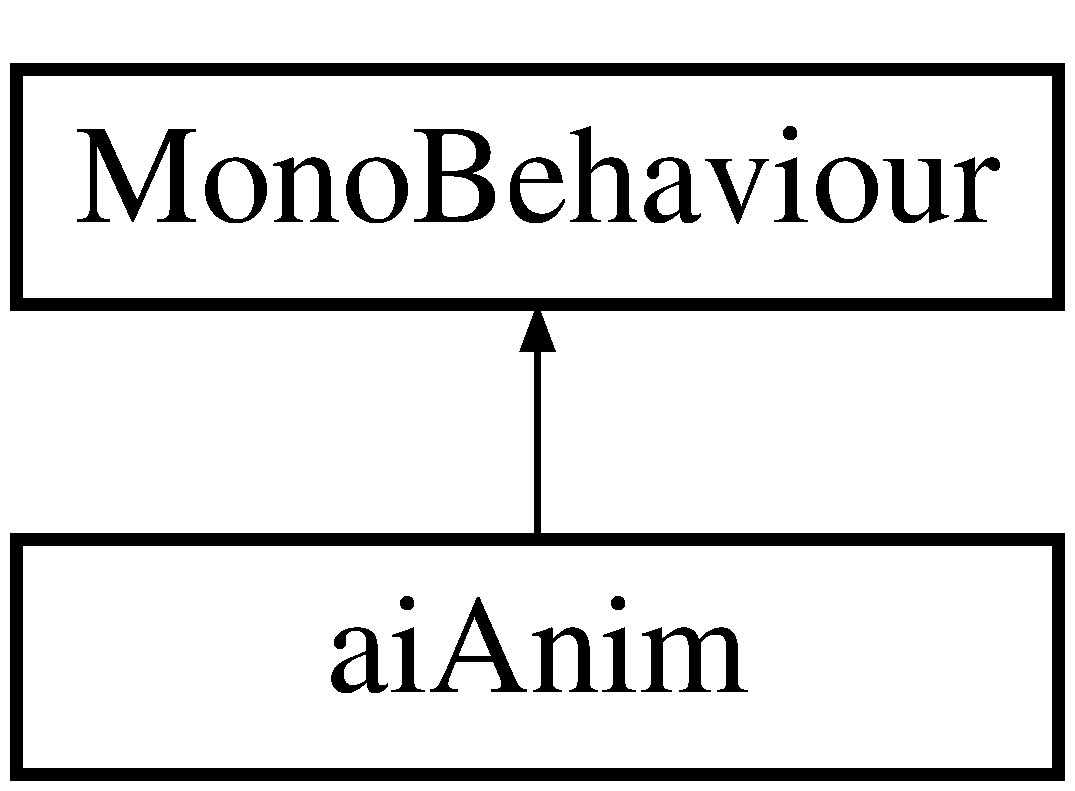
\includegraphics[height=2.000000cm]{classai_anim}
\end{center}
\end{figure}


\subsection{Detailed Description}


Definition at line 13 of file ai\+Anim.\+cs.



The documentation for this class was generated from the following file\+:\begin{DoxyCompactItemize}
\item 
Virus\+Project/\+Assets/\+Scripts/\hyperlink{ai_anim_8cs}{ai\+Anim.\+cs}\end{DoxyCompactItemize}

\hypertarget{class_camera_script}{}\section{Camera\+Script Class Reference}
\label{class_camera_script}\index{Camera\+Script@{Camera\+Script}}
Inheritance diagram for Camera\+Script\+:\begin{figure}[H]
\begin{center}
\leavevmode
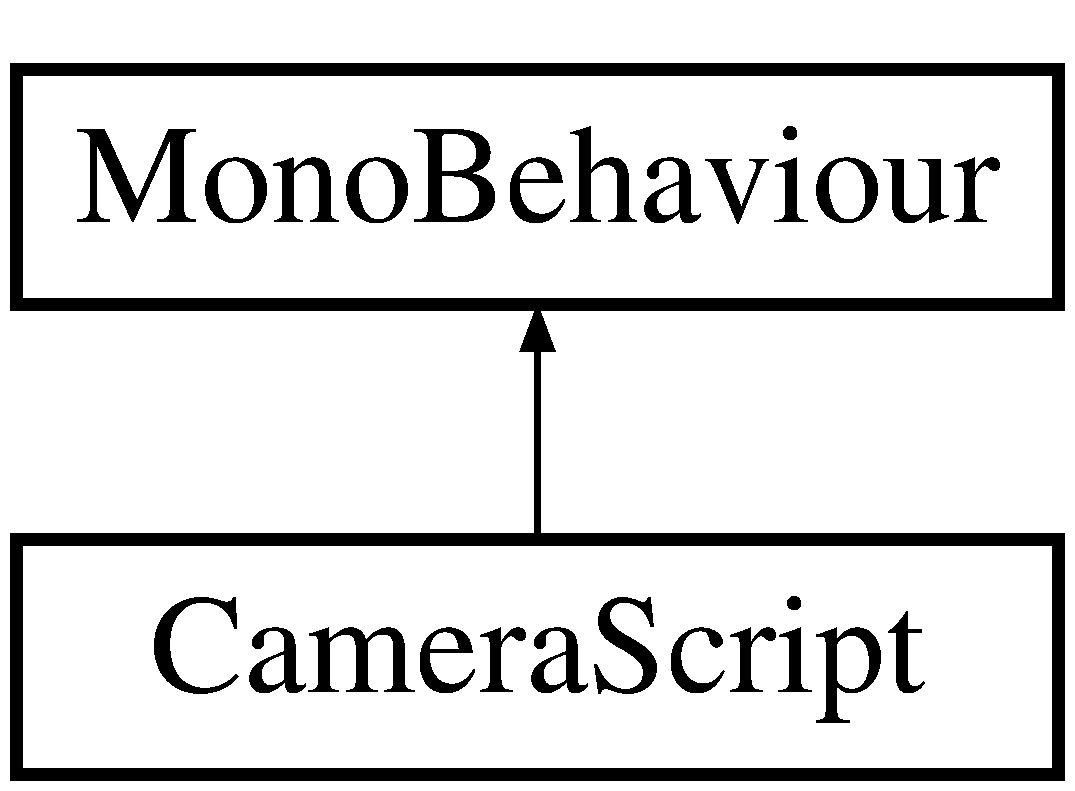
\includegraphics[height=2.000000cm]{class_camera_script}
\end{center}
\end{figure}
\subsection*{Public Attributes}
\begin{DoxyCompactItemize}
\item 
Transform \hyperlink{class_camera_script_a0cb84b0b035c8ef0fd33a9698da77b27}{target}
\item 
float \hyperlink{class_camera_script_ae9f7545052003199e6cc184fe1e1ec29}{distance}
\end{DoxyCompactItemize}


\subsection{Detailed Description}


Definition at line 13 of file Camera\+Script.\+cs.



\subsection{Member Data Documentation}
\hypertarget{class_camera_script_ae9f7545052003199e6cc184fe1e1ec29}{}\label{class_camera_script_ae9f7545052003199e6cc184fe1e1ec29} 
\index{Camera\+Script@{Camera\+Script}!distance@{distance}}
\index{distance@{distance}!Camera\+Script@{Camera\+Script}}
\subsubsection{\texorpdfstring{distance}{distance}}
{\footnotesize\ttfamily float Camera\+Script.\+distance}



Definition at line 19 of file Camera\+Script.\+cs.

\hypertarget{class_camera_script_a0cb84b0b035c8ef0fd33a9698da77b27}{}\label{class_camera_script_a0cb84b0b035c8ef0fd33a9698da77b27} 
\index{Camera\+Script@{Camera\+Script}!target@{target}}
\index{target@{target}!Camera\+Script@{Camera\+Script}}
\subsubsection{\texorpdfstring{target}{target}}
{\footnotesize\ttfamily Transform Camera\+Script.\+target}



Definition at line 16 of file Camera\+Script.\+cs.



The documentation for this class was generated from the following file\+:\begin{DoxyCompactItemize}
\item 
Virus\+Project/\+Assets/\+Scripts/\hyperlink{_camera_script_8cs}{Camera\+Script.\+cs}\end{DoxyCompactItemize}

\hypertarget{classdestination_talk}{}\section{destination\+Talk Class Reference}
\label{classdestination_talk}\index{destination\+Talk@{destination\+Talk}}
Inheritance diagram for destination\+Talk\+:\begin{figure}[H]
\begin{center}
\leavevmode
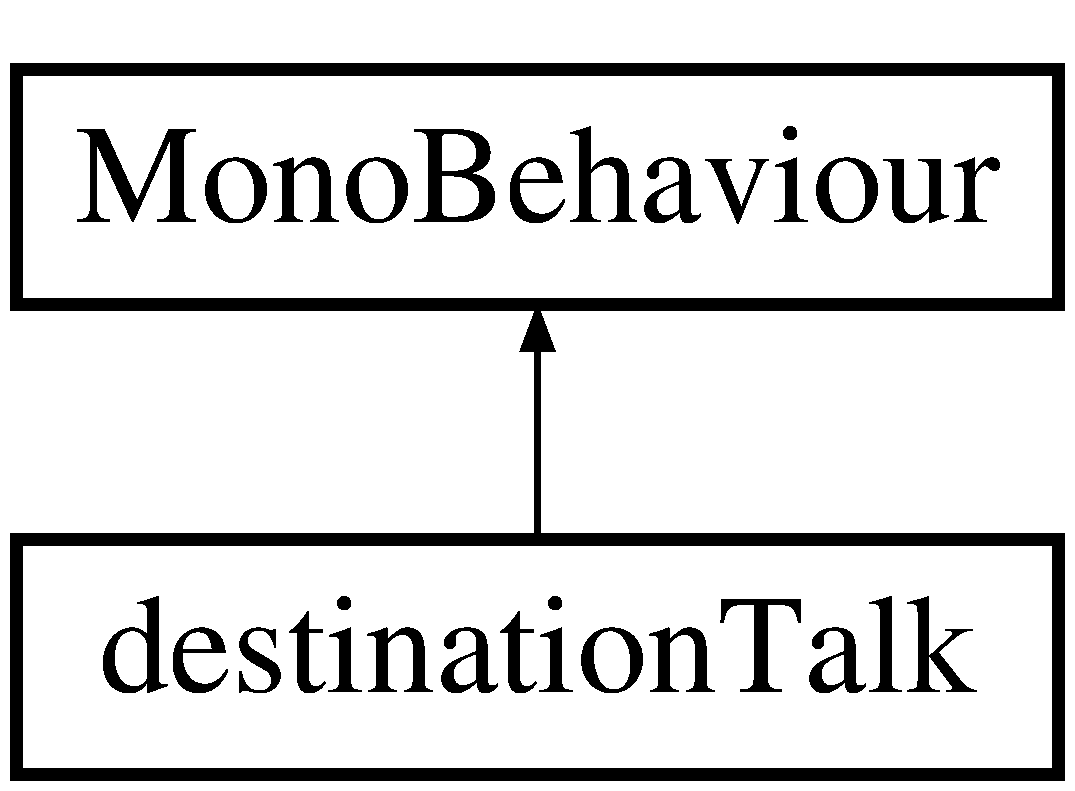
\includegraphics[height=2.000000cm]{classdestination_talk}
\end{center}
\end{figure}
\subsection*{Public Attributes}
\begin{DoxyCompactItemize}
\item 
bool \hyperlink{classdestination_talk_aa9bf6e6e6c6d707c5aa33de9afa0c947}{talk}
\end{DoxyCompactItemize}


\subsection{Detailed Description}


Definition at line 13 of file destination\+Talk.\+cs.



\subsection{Member Data Documentation}
\hypertarget{classdestination_talk_aa9bf6e6e6c6d707c5aa33de9afa0c947}{}\label{classdestination_talk_aa9bf6e6e6c6d707c5aa33de9afa0c947} 
\index{destination\+Talk@{destination\+Talk}!talk@{talk}}
\index{talk@{talk}!destination\+Talk@{destination\+Talk}}
\subsubsection{\texorpdfstring{talk}{talk}}
{\footnotesize\ttfamily bool destination\+Talk.\+talk}



Definition at line 16 of file destination\+Talk.\+cs.



The documentation for this class was generated from the following file\+:\begin{DoxyCompactItemize}
\item 
Virus\+Project/\+Assets/\+Scripts/\hyperlink{destination_talk_8cs}{destination\+Talk.\+cs}\end{DoxyCompactItemize}

\hypertarget{classsim_person_1_1_dest_slot}{}\section{sim\+Person.\+Dest\+Slot Class Reference}
\label{classsim_person_1_1_dest_slot}\index{sim\+Person.\+Dest\+Slot@{sim\+Person.\+Dest\+Slot}}
Inheritance diagram for sim\+Person.\+Dest\+Slot\+:\begin{figure}[H]
\begin{center}
\leavevmode
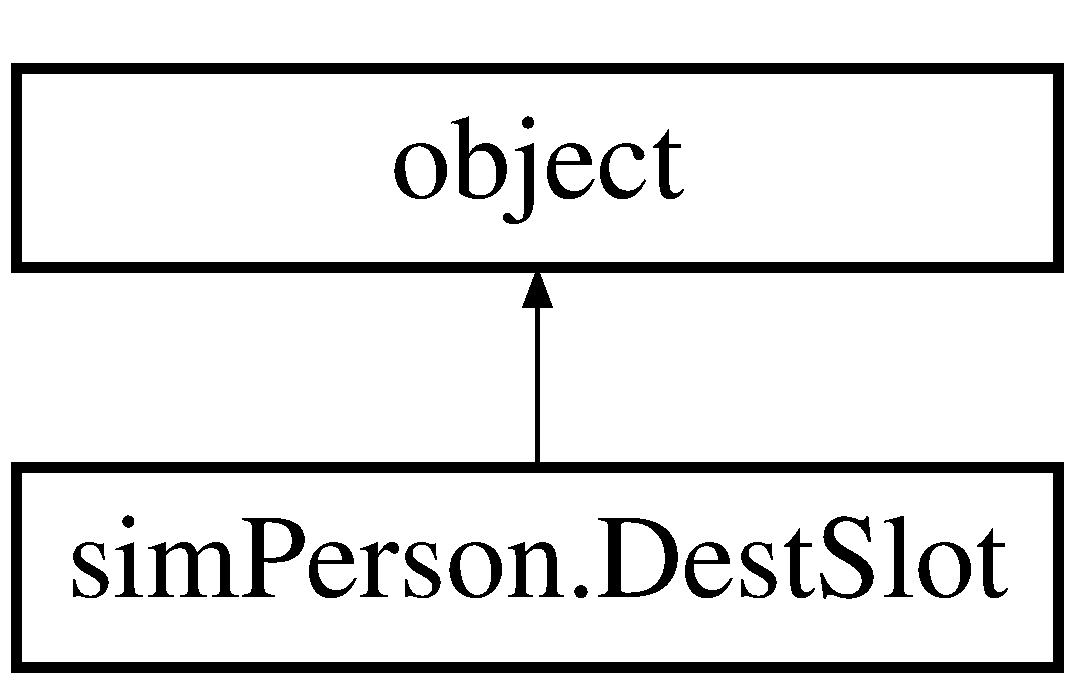
\includegraphics[height=2.000000cm]{classsim_person_1_1_dest_slot}
\end{center}
\end{figure}
\subsection*{Public Member Functions}
\begin{DoxyCompactItemize}
\item 
\hyperlink{classsim_person_1_1_dest_slot_aa6596787998f78f3f15dc8de2a7a3ede}{Dest\+Slot} (int dest, int wait\+Time)
\item 
override bool \hyperlink{classsim_person_1_1_dest_slot_a212d339d7ee8672bea7c06e3ce09a9a4}{Equals} (object obj)
\item 
bool \hyperlink{classsim_person_1_1_dest_slot_abda5a5382912f7eaa87ae75363a9cd81}{Equals} (\hyperlink{classsim_person_1_1_dest_slot}{Dest\+Slot} des)
\item 
override string \hyperlink{classsim_person_1_1_dest_slot_acc639bb6bf443fc68c0c591e5440c3de}{To\+String} ()
\item 
override int \hyperlink{classsim_person_1_1_dest_slot_aedbbf932f62b4aae95b842ebd5519d84}{Get\+Hash\+Code} ()
\end{DoxyCompactItemize}
\subsection*{Properties}
\begin{DoxyCompactItemize}
\item 
int \hyperlink{classsim_person_1_1_dest_slot_ab8e2c3efcdc50551870cb472ea4dc85b}{Dest}\hspace{0.3cm}{\ttfamily  \mbox{[}get, set\mbox{]}}
\item 
int \hyperlink{classsim_person_1_1_dest_slot_a6ab5b25156f6631d1e3b5c66e274f0d3}{Wait\+Time}\hspace{0.3cm}{\ttfamily  \mbox{[}get, set\mbox{]}}
\end{DoxyCompactItemize}


\subsection{Detailed Description}
Virus Simulation Project -\/ Software Engineering Comp 350 \hyperlink{sim_person_8cs}{sim\+Person.\+cs} Purpose\+: Holds information about the destination slots used to queue patrol points for AI. Including Dest as an int and the wait\+Time for each destination.

\begin{DoxyAuthor}{Author}
Joshua Steward 
\end{DoxyAuthor}
\begin{DoxyVersion}{Version}
1.\+0 11/7/2016 
\end{DoxyVersion}


Definition at line 89 of file sim\+Person.\+cs.



\subsection{Constructor \& Destructor Documentation}
\hypertarget{classsim_person_1_1_dest_slot_aa6596787998f78f3f15dc8de2a7a3ede}{}\label{classsim_person_1_1_dest_slot_aa6596787998f78f3f15dc8de2a7a3ede} 
\index{sim\+Person\+::\+Dest\+Slot@{sim\+Person\+::\+Dest\+Slot}!Dest\+Slot@{Dest\+Slot}}
\index{Dest\+Slot@{Dest\+Slot}!sim\+Person\+::\+Dest\+Slot@{sim\+Person\+::\+Dest\+Slot}}
\subsubsection{\texorpdfstring{Dest\+Slot()}{DestSlot()}}
{\footnotesize\ttfamily sim\+Person.\+Dest\+Slot.\+Dest\+Slot (\begin{DoxyParamCaption}\item[{int}]{dest,  }\item[{int}]{wait\+Time }\end{DoxyParamCaption})}

Constructor for this object


\begin{DoxyParams}{Parameters}
{\em dest} & The destination indicator \\
\hline
{\em wait\+Time} & The wait\+Time for this destination \\
\hline
\end{DoxyParams}


Definition at line 102 of file sim\+Person.\+cs.



\subsection{Member Function Documentation}
\hypertarget{classsim_person_1_1_dest_slot_a212d339d7ee8672bea7c06e3ce09a9a4}{}\label{classsim_person_1_1_dest_slot_a212d339d7ee8672bea7c06e3ce09a9a4} 
\index{sim\+Person\+::\+Dest\+Slot@{sim\+Person\+::\+Dest\+Slot}!Equals@{Equals}}
\index{Equals@{Equals}!sim\+Person\+::\+Dest\+Slot@{sim\+Person\+::\+Dest\+Slot}}
\subsubsection{\texorpdfstring{Equals()}{Equals()}\hspace{0.1cm}{\footnotesize\ttfamily [1/2]}}
{\footnotesize\ttfamily override bool sim\+Person.\+Dest\+Slot.\+Equals (\begin{DoxyParamCaption}\item[{object}]{obj }\end{DoxyParamCaption})}

Will compare two destination slots for equality


\begin{DoxyParams}{Parameters}
{\em obj} & The obj to compare for equality \\
\hline
\end{DoxyParams}
\begin{DoxyReturn}{Returns}
bool Equality 
\end{DoxyReturn}


Definition at line 114 of file sim\+Person.\+cs.

\hypertarget{classsim_person_1_1_dest_slot_abda5a5382912f7eaa87ae75363a9cd81}{}\label{classsim_person_1_1_dest_slot_abda5a5382912f7eaa87ae75363a9cd81} 
\index{sim\+Person\+::\+Dest\+Slot@{sim\+Person\+::\+Dest\+Slot}!Equals@{Equals}}
\index{Equals@{Equals}!sim\+Person\+::\+Dest\+Slot@{sim\+Person\+::\+Dest\+Slot}}
\subsubsection{\texorpdfstring{Equals()}{Equals()}\hspace{0.1cm}{\footnotesize\ttfamily [2/2]}}
{\footnotesize\ttfamily bool sim\+Person.\+Dest\+Slot.\+Equals (\begin{DoxyParamCaption}\item[{\hyperlink{classsim_person_1_1_dest_slot}{Dest\+Slot}}]{des }\end{DoxyParamCaption})}

Will compare two destination slots for equality (overrider)


\begin{DoxyParams}{Parameters}
{\em des} & The obj to compare for equality \\
\hline
\end{DoxyParams}
\begin{DoxyReturn}{Returns}
bool Equality 
\end{DoxyReturn}


Definition at line 136 of file sim\+Person.\+cs.

\hypertarget{classsim_person_1_1_dest_slot_aedbbf932f62b4aae95b842ebd5519d84}{}\label{classsim_person_1_1_dest_slot_aedbbf932f62b4aae95b842ebd5519d84} 
\index{sim\+Person\+::\+Dest\+Slot@{sim\+Person\+::\+Dest\+Slot}!Get\+Hash\+Code@{Get\+Hash\+Code}}
\index{Get\+Hash\+Code@{Get\+Hash\+Code}!sim\+Person\+::\+Dest\+Slot@{sim\+Person\+::\+Dest\+Slot}}
\subsubsection{\texorpdfstring{Get\+Hash\+Code()}{GetHashCode()}}
{\footnotesize\ttfamily override int sim\+Person.\+Dest\+Slot.\+Get\+Hash\+Code (\begin{DoxyParamCaption}{ }\end{DoxyParamCaption})}

Will compare two destination slots for equality

\begin{DoxyReturn}{Returns}
hash The hashed slaying hasher of the hash code 
\end{DoxyReturn}


Definition at line 162 of file sim\+Person.\+cs.

\hypertarget{classsim_person_1_1_dest_slot_acc639bb6bf443fc68c0c591e5440c3de}{}\label{classsim_person_1_1_dest_slot_acc639bb6bf443fc68c0c591e5440c3de} 
\index{sim\+Person\+::\+Dest\+Slot@{sim\+Person\+::\+Dest\+Slot}!To\+String@{To\+String}}
\index{To\+String@{To\+String}!sim\+Person\+::\+Dest\+Slot@{sim\+Person\+::\+Dest\+Slot}}
\subsubsection{\texorpdfstring{To\+String()}{ToString()}}
{\footnotesize\ttfamily override string sim\+Person.\+Dest\+Slot.\+To\+String (\begin{DoxyParamCaption}{ }\end{DoxyParamCaption})}

Converts object to string form

\begin{DoxyReturn}{Returns}
string String form of \hyperlink{classsim_person_1_1_dest_slot}{Dest\+Slot} 
\end{DoxyReturn}


Definition at line 151 of file sim\+Person.\+cs.



\subsection{Property Documentation}
\hypertarget{classsim_person_1_1_dest_slot_ab8e2c3efcdc50551870cb472ea4dc85b}{}\label{classsim_person_1_1_dest_slot_ab8e2c3efcdc50551870cb472ea4dc85b} 
\index{sim\+Person\+::\+Dest\+Slot@{sim\+Person\+::\+Dest\+Slot}!Dest@{Dest}}
\index{Dest@{Dest}!sim\+Person\+::\+Dest\+Slot@{sim\+Person\+::\+Dest\+Slot}}
\subsubsection{\texorpdfstring{Dest}{Dest}}
{\footnotesize\ttfamily int sim\+Person.\+Dest\+Slot.\+Dest\hspace{0.3cm}{\ttfamily [get]}, {\ttfamily [set]}}



Definition at line 92 of file sim\+Person.\+cs.

\hypertarget{classsim_person_1_1_dest_slot_a6ab5b25156f6631d1e3b5c66e274f0d3}{}\label{classsim_person_1_1_dest_slot_a6ab5b25156f6631d1e3b5c66e274f0d3} 
\index{sim\+Person\+::\+Dest\+Slot@{sim\+Person\+::\+Dest\+Slot}!Wait\+Time@{Wait\+Time}}
\index{Wait\+Time@{Wait\+Time}!sim\+Person\+::\+Dest\+Slot@{sim\+Person\+::\+Dest\+Slot}}
\subsubsection{\texorpdfstring{Wait\+Time}{WaitTime}}
{\footnotesize\ttfamily int sim\+Person.\+Dest\+Slot.\+Wait\+Time\hspace{0.3cm}{\ttfamily [get]}, {\ttfamily [set]}}



Definition at line 94 of file sim\+Person.\+cs.



The documentation for this class was generated from the following file\+:\begin{DoxyCompactItemize}
\item 
Virus\+Project/\+Assets/\+Scripts/\hyperlink{sim_person_8cs}{sim\+Person.\+cs}\end{DoxyCompactItemize}

\hypertarget{class_display_text}{}\section{Display\+Text Class Reference}
\label{class_display_text}\index{Display\+Text@{Display\+Text}}
Inheritance diagram for Display\+Text\+:\begin{figure}[H]
\begin{center}
\leavevmode
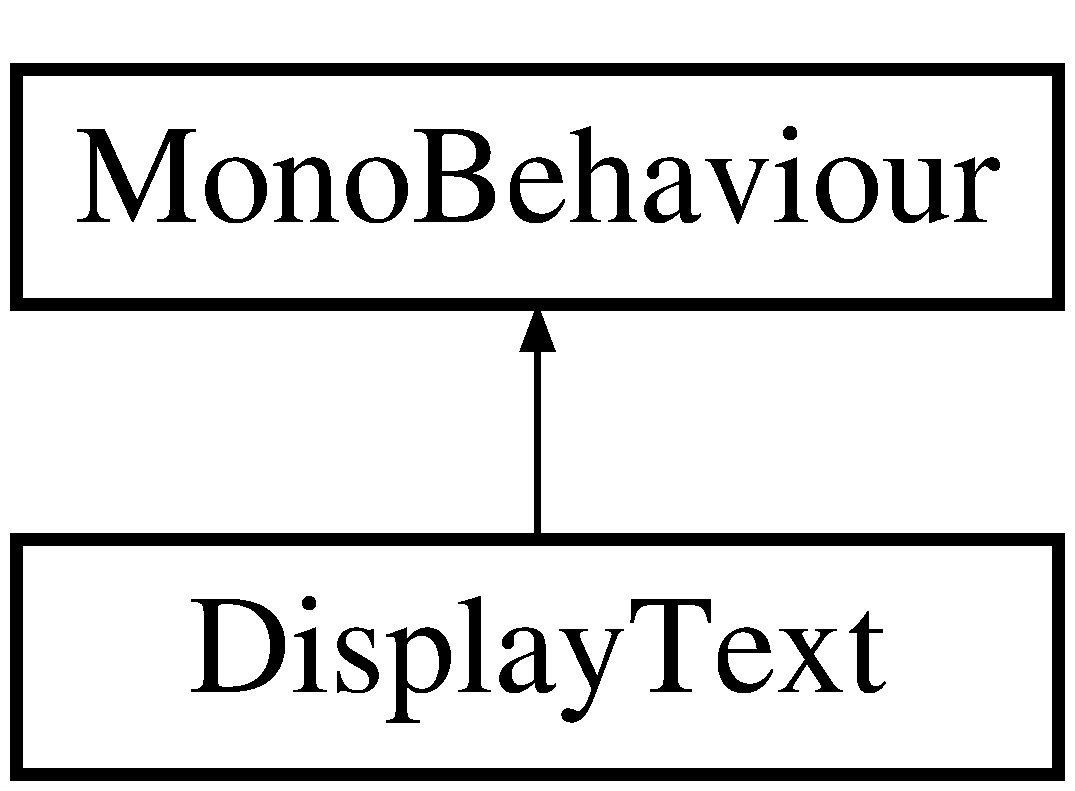
\includegraphics[height=2.000000cm]{class_display_text}
\end{center}
\end{figure}
\subsection*{Public Attributes}
\begin{DoxyCompactItemize}
\item 
string \hyperlink{class_display_text_af937617cbc62e0c9065018c4ab9f7aff}{destination\+Tag}
\item 
float \hyperlink{class_display_text_a284398d2c2ca647b4828d384496447ba}{range}
\end{DoxyCompactItemize}


\subsection{Detailed Description}


Definition at line 14 of file Display\+Text.\+cs.



\subsection{Member Data Documentation}
\hypertarget{class_display_text_af937617cbc62e0c9065018c4ab9f7aff}{}\label{class_display_text_af937617cbc62e0c9065018c4ab9f7aff} 
\index{Display\+Text@{Display\+Text}!destination\+Tag@{destination\+Tag}}
\index{destination\+Tag@{destination\+Tag}!Display\+Text@{Display\+Text}}
\subsubsection{\texorpdfstring{destination\+Tag}{destinationTag}}
{\footnotesize\ttfamily string Display\+Text.\+destination\+Tag}



Definition at line 17 of file Display\+Text.\+cs.

\hypertarget{class_display_text_a284398d2c2ca647b4828d384496447ba}{}\label{class_display_text_a284398d2c2ca647b4828d384496447ba} 
\index{Display\+Text@{Display\+Text}!range@{range}}
\index{range@{range}!Display\+Text@{Display\+Text}}
\subsubsection{\texorpdfstring{range}{range}}
{\footnotesize\ttfamily float Display\+Text.\+range}



Definition at line 20 of file Display\+Text.\+cs.



The documentation for this class was generated from the following file\+:\begin{DoxyCompactItemize}
\item 
Virus\+Project/\+Assets/\+Scripts/\hyperlink{_display_text_8cs}{Display\+Text.\+cs}\end{DoxyCompactItemize}

\hypertarget{classface_mouse}{}\section{face\+Mouse Class Reference}
\label{classface_mouse}\index{face\+Mouse@{face\+Mouse}}
Inheritance diagram for face\+Mouse\+:\begin{figure}[H]
\begin{center}
\leavevmode
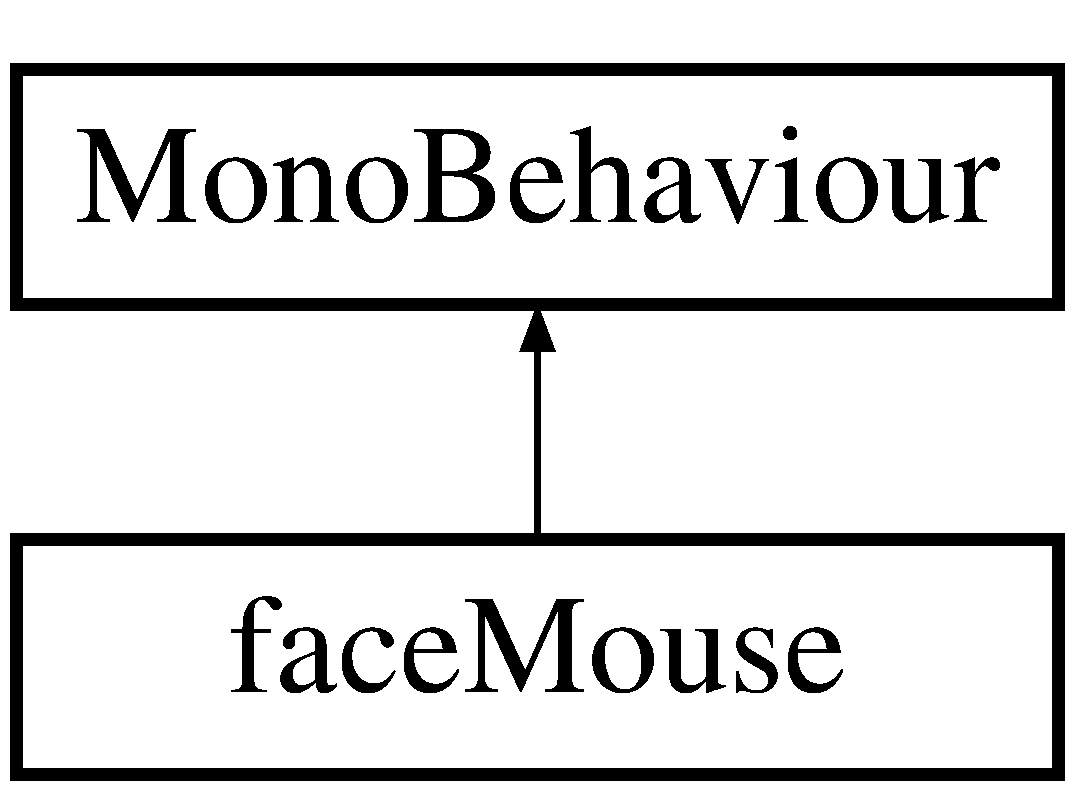
\includegraphics[height=2.000000cm]{classface_mouse}
\end{center}
\end{figure}


\subsection{Detailed Description}


Definition at line 13 of file face\+Mouse.\+cs.



The documentation for this class was generated from the following file\+:\begin{DoxyCompactItemize}
\item 
Virus\+Project/\+Assets/\+Scripts/\hyperlink{face_mouse_8cs}{face\+Mouse.\+cs}\end{DoxyCompactItemize}

\hypertarget{class_game_manager}{}\section{Game\+Manager Class Reference}
\label{class_game_manager}\index{Game\+Manager@{Game\+Manager}}
Inheritance diagram for Game\+Manager\+:\begin{figure}[H]
\begin{center}
\leavevmode
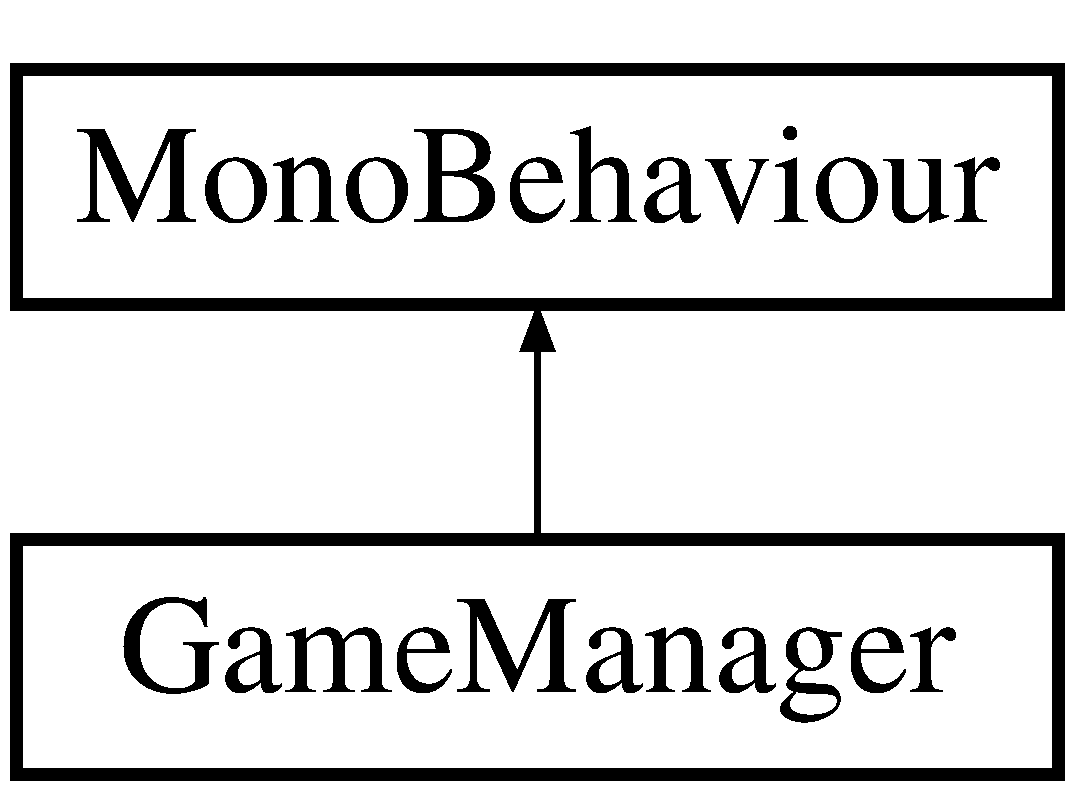
\includegraphics[height=2.000000cm]{class_game_manager}
\end{center}
\end{figure}
\subsection*{Public Attributes}
\begin{DoxyCompactItemize}
\item 
int \hyperlink{class_game_manager_ab49abc66427bbe2c6c1c8a38b58bafae}{count}
\item 
List$<$ Game\+Object $>$ \hyperlink{class_game_manager_ae36910f35ee71379d3f60e9fade57abc}{ai\+List}
\item 
Game\+Object \mbox{[}$\,$\mbox{]} \hyperlink{class_game_manager_a9400f161998957696533cc5e7925d9a1}{destination\+Buildings\+In}
\item 
List$<$ Game\+Object $>$ \hyperlink{class_game_manager_a7207a32a9e7c552a999a850b2bc82579}{dest\+Buildings}
\item 
Text \hyperlink{class_game_manager_a398d163978e15786ef9cea1be1c877d9}{score\+Text}
\end{DoxyCompactItemize}
\subsection*{Static Public Attributes}
\begin{DoxyCompactItemize}
\item 
static \hyperlink{class_game_manager}{Game\+Manager} \hyperlink{class_game_manager_a7666e8468dac197b9eb32dd32128524f}{instance}
\end{DoxyCompactItemize}


\subsection{Detailed Description}


Definition at line 15 of file Game\+Manager.\+cs.



\subsection{Member Data Documentation}
\hypertarget{class_game_manager_ae36910f35ee71379d3f60e9fade57abc}{}\label{class_game_manager_ae36910f35ee71379d3f60e9fade57abc} 
\index{Game\+Manager@{Game\+Manager}!ai\+List@{ai\+List}}
\index{ai\+List@{ai\+List}!Game\+Manager@{Game\+Manager}}
\subsubsection{\texorpdfstring{ai\+List}{aiList}}
{\footnotesize\ttfamily List$<$Game\+Object$>$ Game\+Manager.\+ai\+List}



Definition at line 27 of file Game\+Manager.\+cs.

\hypertarget{class_game_manager_ab49abc66427bbe2c6c1c8a38b58bafae}{}\label{class_game_manager_ab49abc66427bbe2c6c1c8a38b58bafae} 
\index{Game\+Manager@{Game\+Manager}!count@{count}}
\index{count@{count}!Game\+Manager@{Game\+Manager}}
\subsubsection{\texorpdfstring{count}{count}}
{\footnotesize\ttfamily int Game\+Manager.\+count}



Definition at line 21 of file Game\+Manager.\+cs.

\hypertarget{class_game_manager_a7207a32a9e7c552a999a850b2bc82579}{}\label{class_game_manager_a7207a32a9e7c552a999a850b2bc82579} 
\index{Game\+Manager@{Game\+Manager}!dest\+Buildings@{dest\+Buildings}}
\index{dest\+Buildings@{dest\+Buildings}!Game\+Manager@{Game\+Manager}}
\subsubsection{\texorpdfstring{dest\+Buildings}{destBuildings}}
{\footnotesize\ttfamily List$<$Game\+Object$>$ Game\+Manager.\+dest\+Buildings}



Definition at line 36 of file Game\+Manager.\+cs.

\hypertarget{class_game_manager_a9400f161998957696533cc5e7925d9a1}{}\label{class_game_manager_a9400f161998957696533cc5e7925d9a1} 
\index{Game\+Manager@{Game\+Manager}!destination\+Buildings\+In@{destination\+Buildings\+In}}
\index{destination\+Buildings\+In@{destination\+Buildings\+In}!Game\+Manager@{Game\+Manager}}
\subsubsection{\texorpdfstring{destination\+Buildings\+In}{destinationBuildingsIn}}
{\footnotesize\ttfamily Game\+Object \mbox{[}$\,$\mbox{]} Game\+Manager.\+destination\+Buildings\+In}



Definition at line 33 of file Game\+Manager.\+cs.

\hypertarget{class_game_manager_a7666e8468dac197b9eb32dd32128524f}{}\label{class_game_manager_a7666e8468dac197b9eb32dd32128524f} 
\index{Game\+Manager@{Game\+Manager}!instance@{instance}}
\index{instance@{instance}!Game\+Manager@{Game\+Manager}}
\subsubsection{\texorpdfstring{instance}{instance}}
{\footnotesize\ttfamily \hyperlink{class_game_manager}{Game\+Manager} Game\+Manager.\+instance\hspace{0.3cm}{\ttfamily [static]}}



Definition at line 30 of file Game\+Manager.\+cs.

\hypertarget{class_game_manager_a398d163978e15786ef9cea1be1c877d9}{}\label{class_game_manager_a398d163978e15786ef9cea1be1c877d9} 
\index{Game\+Manager@{Game\+Manager}!score\+Text@{score\+Text}}
\index{score\+Text@{score\+Text}!Game\+Manager@{Game\+Manager}}
\subsubsection{\texorpdfstring{score\+Text}{scoreText}}
{\footnotesize\ttfamily Text Game\+Manager.\+score\+Text}



Definition at line 39 of file Game\+Manager.\+cs.



The documentation for this class was generated from the following file\+:\begin{DoxyCompactItemize}
\item 
Virus\+Project/\+Assets/\+Scripts/\hyperlink{_game_manager_8cs}{Game\+Manager.\+cs}\end{DoxyCompactItemize}

\hypertarget{class_infection}{}\section{Infection Class Reference}
\label{class_infection}\index{Infection@{Infection}}
Inheritance diagram for Infection\+:\begin{figure}[H]
\begin{center}
\leavevmode
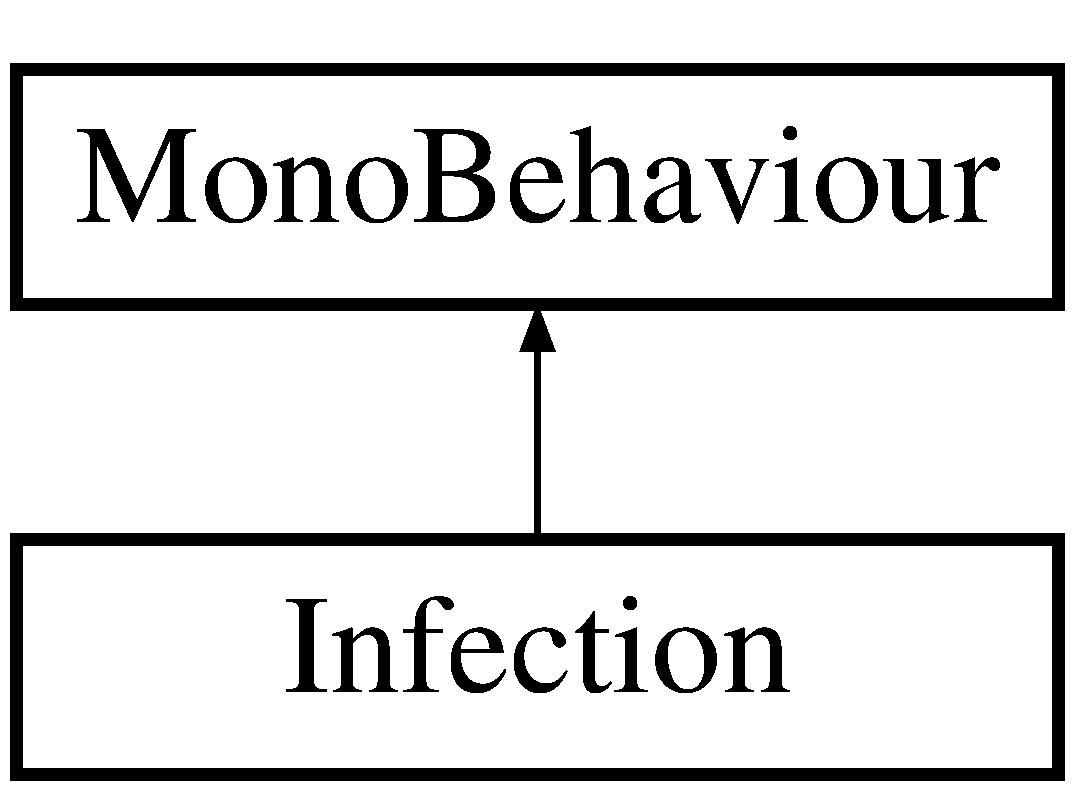
\includegraphics[height=2.000000cm]{class_infection}
\end{center}
\end{figure}
\subsection*{Public Attributes}
\begin{DoxyCompactItemize}
\item 
Game\+Object \hyperlink{class_infection_aac370972b02543b0ad70b25840224f82}{player\+Reference}
\item 
bool \hyperlink{class_infection_ad4b2065e411b4aacb19f2f7ccd32cb47}{infected}
\item 
Color \hyperlink{class_infection_ad3af6c8327fa2602602441aef959bb8f}{current\+Color}
\item 
float \hyperlink{class_infection_ae45fa01c06fe42314a4846d713a436f4}{R}
\item 
float \hyperlink{class_infection_ab3534c9042ed3248a3179d6d3884bf9f}{G}
\item 
float \hyperlink{class_infection_a8fcb6741aa0001114773110539cd9a7a}{B}
\item 
float \hyperlink{class_infection_a7e45ecdc669fde1538935217b430df51}{A}
\end{DoxyCompactItemize}


\subsection{Detailed Description}


Definition at line 16 of file Infection.\+cs.



\subsection{Member Data Documentation}
\hypertarget{class_infection_a7e45ecdc669fde1538935217b430df51}{}\label{class_infection_a7e45ecdc669fde1538935217b430df51} 
\index{Infection@{Infection}!A@{A}}
\index{A@{A}!Infection@{Infection}}
\subsubsection{\texorpdfstring{A}{A}}
{\footnotesize\ttfamily float Infection.\+A}



Definition at line 41 of file Infection.\+cs.

\hypertarget{class_infection_a8fcb6741aa0001114773110539cd9a7a}{}\label{class_infection_a8fcb6741aa0001114773110539cd9a7a} 
\index{Infection@{Infection}!B@{B}}
\index{B@{B}!Infection@{Infection}}
\subsubsection{\texorpdfstring{B}{B}}
{\footnotesize\ttfamily float Infection.\+B}



Definition at line 38 of file Infection.\+cs.

\hypertarget{class_infection_ad3af6c8327fa2602602441aef959bb8f}{}\label{class_infection_ad3af6c8327fa2602602441aef959bb8f} 
\index{Infection@{Infection}!current\+Color@{current\+Color}}
\index{current\+Color@{current\+Color}!Infection@{Infection}}
\subsubsection{\texorpdfstring{current\+Color}{currentColor}}
{\footnotesize\ttfamily Color Infection.\+current\+Color}



Definition at line 26 of file Infection.\+cs.

\hypertarget{class_infection_ab3534c9042ed3248a3179d6d3884bf9f}{}\label{class_infection_ab3534c9042ed3248a3179d6d3884bf9f} 
\index{Infection@{Infection}!G@{G}}
\index{G@{G}!Infection@{Infection}}
\subsubsection{\texorpdfstring{G}{G}}
{\footnotesize\ttfamily float Infection.\+G}



Definition at line 35 of file Infection.\+cs.

\hypertarget{class_infection_ad4b2065e411b4aacb19f2f7ccd32cb47}{}\label{class_infection_ad4b2065e411b4aacb19f2f7ccd32cb47} 
\index{Infection@{Infection}!infected@{infected}}
\index{infected@{infected}!Infection@{Infection}}
\subsubsection{\texorpdfstring{infected}{infected}}
{\footnotesize\ttfamily bool Infection.\+infected}



Definition at line 23 of file Infection.\+cs.

\hypertarget{class_infection_aac370972b02543b0ad70b25840224f82}{}\label{class_infection_aac370972b02543b0ad70b25840224f82} 
\index{Infection@{Infection}!player\+Reference@{player\+Reference}}
\index{player\+Reference@{player\+Reference}!Infection@{Infection}}
\subsubsection{\texorpdfstring{player\+Reference}{playerReference}}
{\footnotesize\ttfamily Game\+Object Infection.\+player\+Reference}



Definition at line 20 of file Infection.\+cs.

\hypertarget{class_infection_ae45fa01c06fe42314a4846d713a436f4}{}\label{class_infection_ae45fa01c06fe42314a4846d713a436f4} 
\index{Infection@{Infection}!R@{R}}
\index{R@{R}!Infection@{Infection}}
\subsubsection{\texorpdfstring{R}{R}}
{\footnotesize\ttfamily float Infection.\+R}



Definition at line 32 of file Infection.\+cs.



The documentation for this class was generated from the following file\+:\begin{DoxyCompactItemize}
\item 
Virus\+Project/\+Assets/\+Scripts/\hyperlink{_infection_8cs}{Infection.\+cs}\end{DoxyCompactItemize}

\hypertarget{classmain_menu}{}\section{main\+Menu Class Reference}
\label{classmain_menu}\index{main\+Menu@{main\+Menu}}
Inheritance diagram for main\+Menu\+:\begin{figure}[H]
\begin{center}
\leavevmode
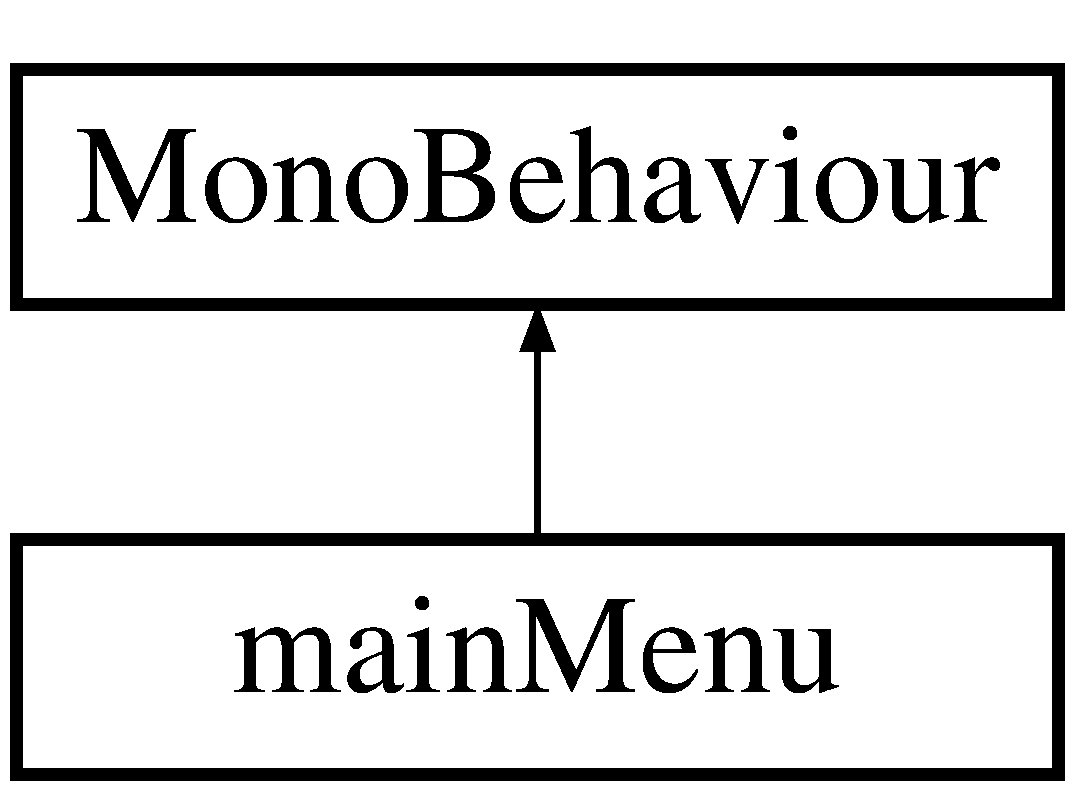
\includegraphics[height=2.000000cm]{classmain_menu}
\end{center}
\end{figure}
\subsection*{Public Member Functions}
\begin{DoxyCompactItemize}
\item 
void \hyperlink{classmain_menu_a5d0b07e8c78863bec5331fa1f307654d}{Load\+By\+Index} (int scene\+Index)
\end{DoxyCompactItemize}


\subsection{Detailed Description}


Definition at line 14 of file main\+Menu.\+cs.



\subsection{Member Function Documentation}
\hypertarget{classmain_menu_a5d0b07e8c78863bec5331fa1f307654d}{}\label{classmain_menu_a5d0b07e8c78863bec5331fa1f307654d} 
\index{main\+Menu@{main\+Menu}!Load\+By\+Index@{Load\+By\+Index}}
\index{Load\+By\+Index@{Load\+By\+Index}!main\+Menu@{main\+Menu}}
\subsubsection{\texorpdfstring{Load\+By\+Index()}{LoadByIndex()}}
{\footnotesize\ttfamily void main\+Menu.\+Load\+By\+Index (\begin{DoxyParamCaption}\item[{int}]{scene\+Index }\end{DoxyParamCaption})}

Will load the main scene.


\begin{DoxyParams}{Parameters}
{\em scene\+Index} & The index in the array of scenes to access \\
\hline
\end{DoxyParams}


Definition at line 22 of file main\+Menu.\+cs.



The documentation for this class was generated from the following file\+:\begin{DoxyCompactItemize}
\item 
Virus\+Project/\+Assets/\+Scripts/\hyperlink{main_menu_8cs}{main\+Menu.\+cs}\end{DoxyCompactItemize}

\hypertarget{classsim_person_1_1_my_state}{}\section{sim\+Person.\+My\+State Class Reference}
\label{classsim_person_1_1_my_state}\index{sim\+Person.\+My\+State@{sim\+Person.\+My\+State}}
\subsection*{Public Member Functions}
\begin{DoxyCompactItemize}
\item 
\hyperlink{classsim_person_1_1_my_state_a574e4fde1a676805dcc1aa580f4b7ed7}{My\+State} (string message, int state)
\end{DoxyCompactItemize}
\subsection*{Properties}
\begin{DoxyCompactItemize}
\item 
string \hyperlink{classsim_person_1_1_my_state_ad0e3e9f33288888b8c76d70b1a78a460}{Message}\hspace{0.3cm}{\ttfamily  \mbox{[}get, set\mbox{]}}
\item 
int \hyperlink{classsim_person_1_1_my_state_a8ea6e800212a919c234ce917b0b75904}{State}\hspace{0.3cm}{\ttfamily  \mbox{[}get, set\mbox{]}}
\end{DoxyCompactItemize}


\subsection{Detailed Description}
Virus Simulation Project -\/ Software Engineering Comp 350 \hyperlink{sim_person_8cs}{sim\+Person.\+cs} Purpose\+: Holds information about the state of the AI

\begin{DoxyAuthor}{Author}
Joshua Steward 
\end{DoxyAuthor}
\begin{DoxyVersion}{Version}
1.\+0 11/7/2016 
\end{DoxyVersion}


Definition at line 178 of file sim\+Person.\+cs.



\subsection{Constructor \& Destructor Documentation}
\hypertarget{classsim_person_1_1_my_state_a574e4fde1a676805dcc1aa580f4b7ed7}{}\label{classsim_person_1_1_my_state_a574e4fde1a676805dcc1aa580f4b7ed7} 
\index{sim\+Person\+::\+My\+State@{sim\+Person\+::\+My\+State}!My\+State@{My\+State}}
\index{My\+State@{My\+State}!sim\+Person\+::\+My\+State@{sim\+Person\+::\+My\+State}}
\subsubsection{\texorpdfstring{My\+State()}{MyState()}}
{\footnotesize\ttfamily sim\+Person.\+My\+State.\+My\+State (\begin{DoxyParamCaption}\item[{string}]{message,  }\item[{int}]{state }\end{DoxyParamCaption})}

Constructor for this object


\begin{DoxyParams}{Parameters}
{\em message} & The string message to be sent \\
\hline
{\em state} & The state of the AI \\
\hline
\end{DoxyParams}


Definition at line 191 of file sim\+Person.\+cs.



\subsection{Property Documentation}
\hypertarget{classsim_person_1_1_my_state_ad0e3e9f33288888b8c76d70b1a78a460}{}\label{classsim_person_1_1_my_state_ad0e3e9f33288888b8c76d70b1a78a460} 
\index{sim\+Person\+::\+My\+State@{sim\+Person\+::\+My\+State}!Message@{Message}}
\index{Message@{Message}!sim\+Person\+::\+My\+State@{sim\+Person\+::\+My\+State}}
\subsubsection{\texorpdfstring{Message}{Message}}
{\footnotesize\ttfamily string sim\+Person.\+My\+State.\+Message\hspace{0.3cm}{\ttfamily [get]}, {\ttfamily [set]}}



Definition at line 181 of file sim\+Person.\+cs.

\hypertarget{classsim_person_1_1_my_state_a8ea6e800212a919c234ce917b0b75904}{}\label{classsim_person_1_1_my_state_a8ea6e800212a919c234ce917b0b75904} 
\index{sim\+Person\+::\+My\+State@{sim\+Person\+::\+My\+State}!State@{State}}
\index{State@{State}!sim\+Person\+::\+My\+State@{sim\+Person\+::\+My\+State}}
\subsubsection{\texorpdfstring{State}{State}}
{\footnotesize\ttfamily int sim\+Person.\+My\+State.\+State\hspace{0.3cm}{\ttfamily [get]}, {\ttfamily [set]}}



Definition at line 183 of file sim\+Person.\+cs.



The documentation for this class was generated from the following file\+:\begin{DoxyCompactItemize}
\item 
Virus\+Project/\+Assets/\+Scripts/\hyperlink{sim_person_8cs}{sim\+Person.\+cs}\end{DoxyCompactItemize}

\hypertarget{class_player_mobility}{}\section{Player\+Mobility Class Reference}
\label{class_player_mobility}\index{Player\+Mobility@{Player\+Mobility}}
Inheritance diagram for Player\+Mobility\+:\begin{figure}[H]
\begin{center}
\leavevmode
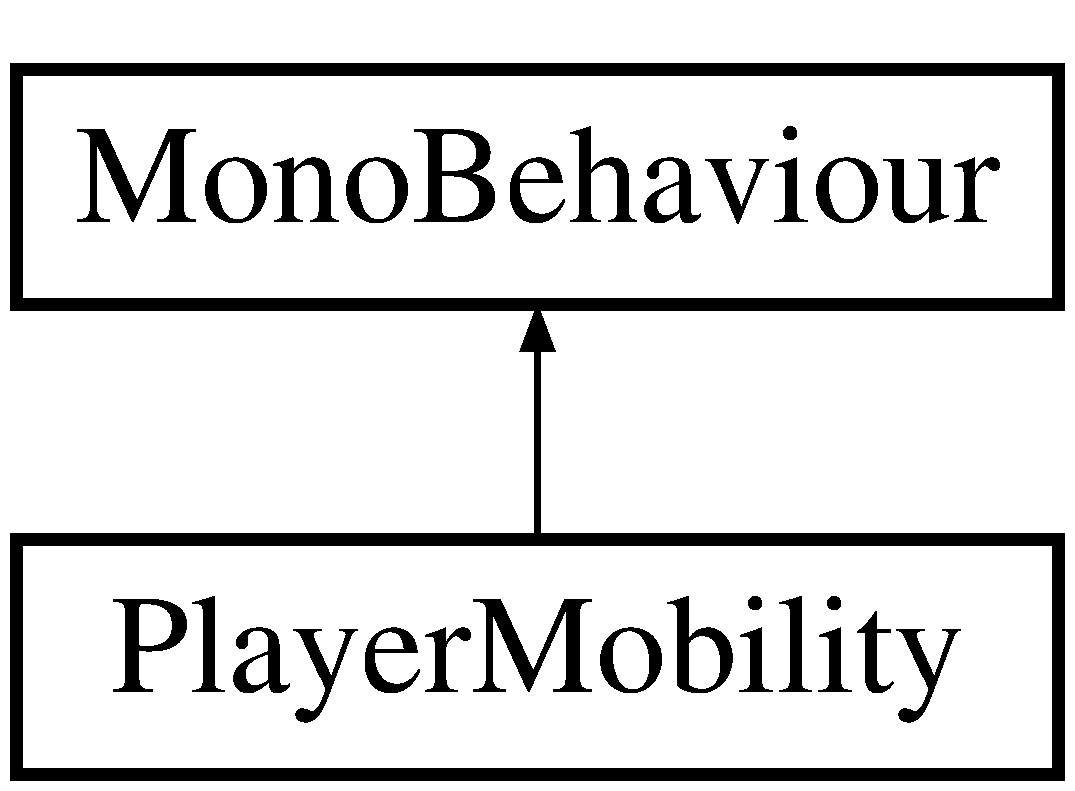
\includegraphics[height=2.000000cm]{class_player_mobility}
\end{center}
\end{figure}
\subsection*{Public Attributes}
\begin{DoxyCompactItemize}
\item 
float \hyperlink{class_player_mobility_a336d35b5a58fc1ea25c0cb8eb88858f0}{speed}
\item 
float \hyperlink{class_player_mobility_aded47b1de0eaf2199854a771f521fe25}{increased\+Speed}
\end{DoxyCompactItemize}


\subsection{Detailed Description}


Definition at line 13 of file Player\+Mobility.\+cs.



\subsection{Member Data Documentation}
\hypertarget{class_player_mobility_aded47b1de0eaf2199854a771f521fe25}{}\label{class_player_mobility_aded47b1de0eaf2199854a771f521fe25} 
\index{Player\+Mobility@{Player\+Mobility}!increased\+Speed@{increased\+Speed}}
\index{increased\+Speed@{increased\+Speed}!Player\+Mobility@{Player\+Mobility}}
\subsubsection{\texorpdfstring{increased\+Speed}{increasedSpeed}}
{\footnotesize\ttfamily float Player\+Mobility.\+increased\+Speed}



Definition at line 23 of file Player\+Mobility.\+cs.

\hypertarget{class_player_mobility_a336d35b5a58fc1ea25c0cb8eb88858f0}{}\label{class_player_mobility_a336d35b5a58fc1ea25c0cb8eb88858f0} 
\index{Player\+Mobility@{Player\+Mobility}!speed@{speed}}
\index{speed@{speed}!Player\+Mobility@{Player\+Mobility}}
\subsubsection{\texorpdfstring{speed}{speed}}
{\footnotesize\ttfamily float Player\+Mobility.\+speed}



Definition at line 17 of file Player\+Mobility.\+cs.



The documentation for this class was generated from the following file\+:\begin{DoxyCompactItemize}
\item 
Virus\+Project/\+Assets/\+Scripts/\hyperlink{_player_mobility_8cs}{Player\+Mobility.\+cs}\end{DoxyCompactItemize}

\hypertarget{classsim_person}{}\section{sim\+Person Class Reference}
\label{classsim_person}\index{sim\+Person@{sim\+Person}}
Inheritance diagram for sim\+Person\+:\begin{figure}[H]
\begin{center}
\leavevmode
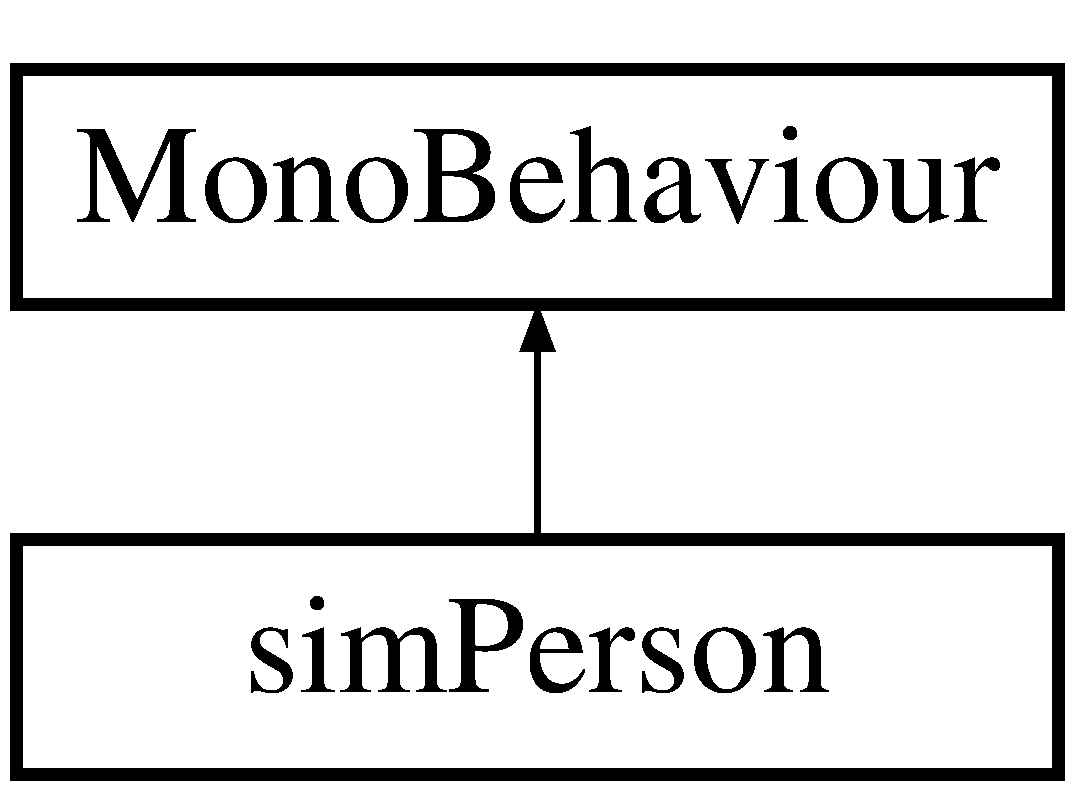
\includegraphics[height=2.000000cm]{classsim_person}
\end{center}
\end{figure}
\subsection*{Classes}
\begin{DoxyCompactItemize}
\item 
class \hyperlink{classsim_person_1_1_dest_slot}{Dest\+Slot}
\item 
class \hyperlink{classsim_person_1_1_my_state}{My\+State}
\end{DoxyCompactItemize}
\subsection*{Public Types}
\begin{DoxyCompactItemize}
\item 
enum \hyperlink{classsim_person_a257596d5b7ccb0179724d7f571cd794d}{Destination} \{ \newline
\hyperlink{classsim_person_a257596d5b7ccb0179724d7f571cd794daaeef646f76c57ed9084edddbb6365b9c}{Destination.\+Club}, 
\hyperlink{classsim_person_a257596d5b7ccb0179724d7f571cd794da72d079ca5ce0fed7a1f448d3a794b15e}{Destination.\+Gamestop}, 
\hyperlink{classsim_person_a257596d5b7ccb0179724d7f571cd794dad04a260b63d40d198636559613ef2c39}{Destination.\+Frys}, 
\hyperlink{classsim_person_a257596d5b7ccb0179724d7f571cd794da0a38e7286ebbb560354992b3ce62be67}{Destination.\+Food}, 
\newline
\hyperlink{classsim_person_a257596d5b7ccb0179724d7f571cd794da7ec9aaa8ac320fa8b83c6f7aaa8c9ca1}{Destination.\+Church}, 
\hyperlink{classsim_person_a257596d5b7ccb0179724d7f571cd794da3c09b8d09553786b799e02306e55c7ba}{Destination.\+Coffee}, 
\hyperlink{classsim_person_a257596d5b7ccb0179724d7f571cd794da8cf04a9734132302f96da8e113e80ce5}{Destination.\+Home}, 
\hyperlink{classsim_person_a257596d5b7ccb0179724d7f571cd794da955cd8691ca89a6baa6ea10c7787e604}{Destination.\+School}
 \}
\item 
enum \hyperlink{classsim_person_a2966469724e979a6aeca2f3b1d40b622}{People\+Type} \{ \newline
\hyperlink{classsim_person_a2966469724e979a6aeca2f3b1d40b622adabdb387ade6712237057f681b38bd12}{People\+Type.\+Nerd}, 
\hyperlink{classsim_person_a2966469724e979a6aeca2f3b1d40b622a0b7fafd9bd19cc911b0499f3e1d73d30}{People\+Type.\+Work\+A\+Holic}, 
\hyperlink{classsim_person_a2966469724e979a6aeca2f3b1d40b622a30269022e9d8f51beaabb52e5d0de2b7}{People\+Type.\+Parent}, 
\hyperlink{classsim_person_a2966469724e979a6aeca2f3b1d40b622aa82fea383f121c803741f8de1c209734}{People\+Type.\+Child}, 
\newline
\hyperlink{classsim_person_a2966469724e979a6aeca2f3b1d40b622aa41523233bdde5831aa45f6b5805ec5c}{People\+Type.\+Habitual\+Eater}, 
\hyperlink{classsim_person_a2966469724e979a6aeca2f3b1d40b622af60dd88837dbc3319c975946d982c8f8}{People\+Type.\+Partier}
 \}
\item 
enum \hyperlink{classsim_person_a2e742c09e6786146fe250d0066fe78e9}{State} \{ \hyperlink{classsim_person_a2e742c09e6786146fe250d0066fe78e9adb6ea77c7cd8a86b17014c3b688fd1a1}{State.\+Walking}, 
\hyperlink{classsim_person_a2e742c09e6786146fe250d0066fe78e9a5706de961fb376d701be6e7762d8b09c}{State.\+Waiting}, 
\hyperlink{classsim_person_a2e742c09e6786146fe250d0066fe78e9a554eee4c195ae0dd1ccafbc75772b951}{State.\+Detection}
 \}
\end{DoxyCompactItemize}
\subsection*{Public Member Functions}
\begin{DoxyCompactItemize}
\item 
void \hyperlink{classsim_person_aca3d90fe7d83818e4ef9b8570b353965}{Patrol} ()
\end{DoxyCompactItemize}
\subsection*{Public Attributes}
\begin{DoxyCompactItemize}
\item 
Transform \hyperlink{classsim_person_a5db445fe5749d0b0165efeb3bd7b0ba9}{target}
\item 
float \hyperlink{classsim_person_a28e2b04758c3682f50ba01eb5d1740c0}{speed}
\item 
int \hyperlink{classsim_person_ac816cec7286f37dc4f4fa30d5c5d909c}{dest\+Capacity}
\item 
\hyperlink{classsim_person_1_1_dest_slot}{Dest\+Slot} \hyperlink{classsim_person_ae3bcceb05ae974887c5f6f68951f5dcc}{next\+Dest}
\item 
Game\+Object \hyperlink{classsim_person_a47b2bb1a902576614f65b7ecf1fa1bdd}{current\+Waypoint}
\item 
\hyperlink{classsim_person_a2e742c09e6786146fe250d0066fe78e9}{State} \hyperlink{classsim_person_aae85299b3299888345288c53bf991626}{my\+State}
\item 
List$<$ \hyperlink{classsim_person_1_1_dest_slot}{Dest\+Slot} $>$ \hyperlink{classsim_person_a1459d9a83816086b302d5fb609855ed7}{my\+Destinations} = new List$<$\hyperlink{classsim_person_1_1_dest_slot}{Dest\+Slot}$>$()
\item 
int \mbox{[}$\,$\mbox{]} \hyperlink{classsim_person_aebd6a40f59fce0a78e71599b0b39bc67}{patrol\+Points}
\item 
string \hyperlink{classsim_person_af45d2902026e35903cebbe51f66caf30}{way\+Point\+Track}
\item 
bool \hyperlink{classsim_person_a21ac457e8040d80854cb5b1ab59bfd6f}{once\+Per\+Cycle} = true
\item 
int \hyperlink{classsim_person_aefacfa94adcf92832728769bb58895bc}{my\+Type}
\end{DoxyCompactItemize}


\subsection{Detailed Description}


Definition at line 16 of file sim\+Person.\+cs.



\subsection{Member Enumeration Documentation}
\hypertarget{classsim_person_a257596d5b7ccb0179724d7f571cd794d}{}\label{classsim_person_a257596d5b7ccb0179724d7f571cd794d} 
\index{sim\+Person@{sim\+Person}!Destination@{Destination}}
\index{Destination@{Destination}!sim\+Person@{sim\+Person}}
\subsubsection{\texorpdfstring{Destination}{Destination}}
{\footnotesize\ttfamily enum \hyperlink{classsim_person_a257596d5b7ccb0179724d7f571cd794d}{sim\+Person.\+Destination}\hspace{0.3cm}{\ttfamily [strong]}}

\begin{DoxyEnumFields}{Enumerator}
\raisebox{\heightof{T}}[0pt][0pt]{\index{Club@{Club}!sim\+Person@{sim\+Person}}\index{sim\+Person@{sim\+Person}!Club@{Club}}}\hypertarget{classsim_person_a257596d5b7ccb0179724d7f571cd794daaeef646f76c57ed9084edddbb6365b9c}{}\label{classsim_person_a257596d5b7ccb0179724d7f571cd794daaeef646f76c57ed9084edddbb6365b9c} 
Club&\\
\hline

\raisebox{\heightof{T}}[0pt][0pt]{\index{Gamestop@{Gamestop}!sim\+Person@{sim\+Person}}\index{sim\+Person@{sim\+Person}!Gamestop@{Gamestop}}}\hypertarget{classsim_person_a257596d5b7ccb0179724d7f571cd794da72d079ca5ce0fed7a1f448d3a794b15e}{}\label{classsim_person_a257596d5b7ccb0179724d7f571cd794da72d079ca5ce0fed7a1f448d3a794b15e} 
Gamestop&\\
\hline

\raisebox{\heightof{T}}[0pt][0pt]{\index{Frys@{Frys}!sim\+Person@{sim\+Person}}\index{sim\+Person@{sim\+Person}!Frys@{Frys}}}\hypertarget{classsim_person_a257596d5b7ccb0179724d7f571cd794dad04a260b63d40d198636559613ef2c39}{}\label{classsim_person_a257596d5b7ccb0179724d7f571cd794dad04a260b63d40d198636559613ef2c39} 
Frys&\\
\hline

\raisebox{\heightof{T}}[0pt][0pt]{\index{Food@{Food}!sim\+Person@{sim\+Person}}\index{sim\+Person@{sim\+Person}!Food@{Food}}}\hypertarget{classsim_person_a257596d5b7ccb0179724d7f571cd794da0a38e7286ebbb560354992b3ce62be67}{}\label{classsim_person_a257596d5b7ccb0179724d7f571cd794da0a38e7286ebbb560354992b3ce62be67} 
Food&\\
\hline

\raisebox{\heightof{T}}[0pt][0pt]{\index{Church@{Church}!sim\+Person@{sim\+Person}}\index{sim\+Person@{sim\+Person}!Church@{Church}}}\hypertarget{classsim_person_a257596d5b7ccb0179724d7f571cd794da7ec9aaa8ac320fa8b83c6f7aaa8c9ca1}{}\label{classsim_person_a257596d5b7ccb0179724d7f571cd794da7ec9aaa8ac320fa8b83c6f7aaa8c9ca1} 
Church&\\
\hline

\raisebox{\heightof{T}}[0pt][0pt]{\index{Coffee@{Coffee}!sim\+Person@{sim\+Person}}\index{sim\+Person@{sim\+Person}!Coffee@{Coffee}}}\hypertarget{classsim_person_a257596d5b7ccb0179724d7f571cd794da3c09b8d09553786b799e02306e55c7ba}{}\label{classsim_person_a257596d5b7ccb0179724d7f571cd794da3c09b8d09553786b799e02306e55c7ba} 
Coffee&\\
\hline

\raisebox{\heightof{T}}[0pt][0pt]{\index{Home@{Home}!sim\+Person@{sim\+Person}}\index{sim\+Person@{sim\+Person}!Home@{Home}}}\hypertarget{classsim_person_a257596d5b7ccb0179724d7f571cd794da8cf04a9734132302f96da8e113e80ce5}{}\label{classsim_person_a257596d5b7ccb0179724d7f571cd794da8cf04a9734132302f96da8e113e80ce5} 
Home&\\
\hline

\raisebox{\heightof{T}}[0pt][0pt]{\index{School@{School}!sim\+Person@{sim\+Person}}\index{sim\+Person@{sim\+Person}!School@{School}}}\hypertarget{classsim_person_a257596d5b7ccb0179724d7f571cd794da955cd8691ca89a6baa6ea10c7787e604}{}\label{classsim_person_a257596d5b7ccb0179724d7f571cd794da955cd8691ca89a6baa6ea10c7787e604} 
School&\\
\hline

\end{DoxyEnumFields}


Definition at line 41 of file sim\+Person.\+cs.

\hypertarget{classsim_person_a2966469724e979a6aeca2f3b1d40b622}{}\label{classsim_person_a2966469724e979a6aeca2f3b1d40b622} 
\index{sim\+Person@{sim\+Person}!People\+Type@{People\+Type}}
\index{People\+Type@{People\+Type}!sim\+Person@{sim\+Person}}
\subsubsection{\texorpdfstring{People\+Type}{PeopleType}}
{\footnotesize\ttfamily enum \hyperlink{classsim_person_a2966469724e979a6aeca2f3b1d40b622}{sim\+Person.\+People\+Type}\hspace{0.3cm}{\ttfamily [strong]}}

\begin{DoxyEnumFields}{Enumerator}
\raisebox{\heightof{T}}[0pt][0pt]{\index{Nerd@{Nerd}!sim\+Person@{sim\+Person}}\index{sim\+Person@{sim\+Person}!Nerd@{Nerd}}}\hypertarget{classsim_person_a2966469724e979a6aeca2f3b1d40b622adabdb387ade6712237057f681b38bd12}{}\label{classsim_person_a2966469724e979a6aeca2f3b1d40b622adabdb387ade6712237057f681b38bd12} 
Nerd&\\
\hline

\raisebox{\heightof{T}}[0pt][0pt]{\index{Work\+A\+Holic@{Work\+A\+Holic}!sim\+Person@{sim\+Person}}\index{sim\+Person@{sim\+Person}!Work\+A\+Holic@{Work\+A\+Holic}}}\hypertarget{classsim_person_a2966469724e979a6aeca2f3b1d40b622a0b7fafd9bd19cc911b0499f3e1d73d30}{}\label{classsim_person_a2966469724e979a6aeca2f3b1d40b622a0b7fafd9bd19cc911b0499f3e1d73d30} 
Work\+A\+Holic&\\
\hline

\raisebox{\heightof{T}}[0pt][0pt]{\index{Parent@{Parent}!sim\+Person@{sim\+Person}}\index{sim\+Person@{sim\+Person}!Parent@{Parent}}}\hypertarget{classsim_person_a2966469724e979a6aeca2f3b1d40b622a30269022e9d8f51beaabb52e5d0de2b7}{}\label{classsim_person_a2966469724e979a6aeca2f3b1d40b622a30269022e9d8f51beaabb52e5d0de2b7} 
Parent&\\
\hline

\raisebox{\heightof{T}}[0pt][0pt]{\index{Child@{Child}!sim\+Person@{sim\+Person}}\index{sim\+Person@{sim\+Person}!Child@{Child}}}\hypertarget{classsim_person_a2966469724e979a6aeca2f3b1d40b622aa82fea383f121c803741f8de1c209734}{}\label{classsim_person_a2966469724e979a6aeca2f3b1d40b622aa82fea383f121c803741f8de1c209734} 
Child&\\
\hline

\raisebox{\heightof{T}}[0pt][0pt]{\index{Habitual\+Eater@{Habitual\+Eater}!sim\+Person@{sim\+Person}}\index{sim\+Person@{sim\+Person}!Habitual\+Eater@{Habitual\+Eater}}}\hypertarget{classsim_person_a2966469724e979a6aeca2f3b1d40b622aa41523233bdde5831aa45f6b5805ec5c}{}\label{classsim_person_a2966469724e979a6aeca2f3b1d40b622aa41523233bdde5831aa45f6b5805ec5c} 
Habitual\+Eater&\\
\hline

\raisebox{\heightof{T}}[0pt][0pt]{\index{Partier@{Partier}!sim\+Person@{sim\+Person}}\index{sim\+Person@{sim\+Person}!Partier@{Partier}}}\hypertarget{classsim_person_a2966469724e979a6aeca2f3b1d40b622af60dd88837dbc3319c975946d982c8f8}{}\label{classsim_person_a2966469724e979a6aeca2f3b1d40b622af60dd88837dbc3319c975946d982c8f8} 
Partier&\\
\hline

\end{DoxyEnumFields}


Definition at line 47 of file sim\+Person.\+cs.

\hypertarget{classsim_person_a2e742c09e6786146fe250d0066fe78e9}{}\label{classsim_person_a2e742c09e6786146fe250d0066fe78e9} 
\index{sim\+Person@{sim\+Person}!State@{State}}
\index{State@{State}!sim\+Person@{sim\+Person}}
\subsubsection{\texorpdfstring{State}{State}}
{\footnotesize\ttfamily enum \hyperlink{classsim_person_a2e742c09e6786146fe250d0066fe78e9}{sim\+Person.\+State}\hspace{0.3cm}{\ttfamily [strong]}}

\begin{DoxyEnumFields}{Enumerator}
\raisebox{\heightof{T}}[0pt][0pt]{\index{Walking@{Walking}!sim\+Person@{sim\+Person}}\index{sim\+Person@{sim\+Person}!Walking@{Walking}}}\hypertarget{classsim_person_a2e742c09e6786146fe250d0066fe78e9adb6ea77c7cd8a86b17014c3b688fd1a1}{}\label{classsim_person_a2e742c09e6786146fe250d0066fe78e9adb6ea77c7cd8a86b17014c3b688fd1a1} 
Walking&\\
\hline

\raisebox{\heightof{T}}[0pt][0pt]{\index{Waiting@{Waiting}!sim\+Person@{sim\+Person}}\index{sim\+Person@{sim\+Person}!Waiting@{Waiting}}}\hypertarget{classsim_person_a2e742c09e6786146fe250d0066fe78e9a5706de961fb376d701be6e7762d8b09c}{}\label{classsim_person_a2e742c09e6786146fe250d0066fe78e9a5706de961fb376d701be6e7762d8b09c} 
Waiting&\\
\hline

\raisebox{\heightof{T}}[0pt][0pt]{\index{Detection@{Detection}!sim\+Person@{sim\+Person}}\index{sim\+Person@{sim\+Person}!Detection@{Detection}}}\hypertarget{classsim_person_a2e742c09e6786146fe250d0066fe78e9a554eee4c195ae0dd1ccafbc75772b951}{}\label{classsim_person_a2e742c09e6786146fe250d0066fe78e9a554eee4c195ae0dd1ccafbc75772b951} 
Detection&\\
\hline

\end{DoxyEnumFields}


Definition at line 53 of file sim\+Person.\+cs.



\subsection{Member Function Documentation}
\hypertarget{classsim_person_aca3d90fe7d83818e4ef9b8570b353965}{}\label{classsim_person_aca3d90fe7d83818e4ef9b8570b353965} 
\index{sim\+Person@{sim\+Person}!Patrol@{Patrol}}
\index{Patrol@{Patrol}!sim\+Person@{sim\+Person}}
\subsubsection{\texorpdfstring{Patrol()}{Patrol()}}
{\footnotesize\ttfamily void sim\+Person.\+Patrol (\begin{DoxyParamCaption}{ }\end{DoxyParamCaption})}

Sets pathfinding class variables, speeds, and compares to destination. On quick transitions between destinations and states, will run a test to make sure there are destinations available. 

Definition at line 288 of file sim\+Person.\+cs.



\subsection{Member Data Documentation}
\hypertarget{classsim_person_a47b2bb1a902576614f65b7ecf1fa1bdd}{}\label{classsim_person_a47b2bb1a902576614f65b7ecf1fa1bdd} 
\index{sim\+Person@{sim\+Person}!current\+Waypoint@{current\+Waypoint}}
\index{current\+Waypoint@{current\+Waypoint}!sim\+Person@{sim\+Person}}
\subsubsection{\texorpdfstring{current\+Waypoint}{currentWaypoint}}
{\footnotesize\ttfamily Game\+Object sim\+Person.\+current\+Waypoint}



Definition at line 38 of file sim\+Person.\+cs.

\hypertarget{classsim_person_ac816cec7286f37dc4f4fa30d5c5d909c}{}\label{classsim_person_ac816cec7286f37dc4f4fa30d5c5d909c} 
\index{sim\+Person@{sim\+Person}!dest\+Capacity@{dest\+Capacity}}
\index{dest\+Capacity@{dest\+Capacity}!sim\+Person@{sim\+Person}}
\subsubsection{\texorpdfstring{dest\+Capacity}{destCapacity}}
{\footnotesize\ttfamily int sim\+Person.\+dest\+Capacity}



Definition at line 32 of file sim\+Person.\+cs.

\hypertarget{classsim_person_a1459d9a83816086b302d5fb609855ed7}{}\label{classsim_person_a1459d9a83816086b302d5fb609855ed7} 
\index{sim\+Person@{sim\+Person}!my\+Destinations@{my\+Destinations}}
\index{my\+Destinations@{my\+Destinations}!sim\+Person@{sim\+Person}}
\subsubsection{\texorpdfstring{my\+Destinations}{myDestinations}}
{\footnotesize\ttfamily List$<$\hyperlink{classsim_person_1_1_dest_slot}{Dest\+Slot}$>$ sim\+Person.\+my\+Destinations = new List$<$\hyperlink{classsim_person_1_1_dest_slot}{Dest\+Slot}$>$()}



Definition at line 62 of file sim\+Person.\+cs.

\hypertarget{classsim_person_aae85299b3299888345288c53bf991626}{}\label{classsim_person_aae85299b3299888345288c53bf991626} 
\index{sim\+Person@{sim\+Person}!my\+State@{my\+State}}
\index{my\+State@{my\+State}!sim\+Person@{sim\+Person}}
\subsubsection{\texorpdfstring{my\+State}{myState}}
{\footnotesize\ttfamily \hyperlink{classsim_person_a2e742c09e6786146fe250d0066fe78e9}{State} sim\+Person.\+my\+State}



Definition at line 56 of file sim\+Person.\+cs.

\hypertarget{classsim_person_aefacfa94adcf92832728769bb58895bc}{}\label{classsim_person_aefacfa94adcf92832728769bb58895bc} 
\index{sim\+Person@{sim\+Person}!my\+Type@{my\+Type}}
\index{my\+Type@{my\+Type}!sim\+Person@{sim\+Person}}
\subsubsection{\texorpdfstring{my\+Type}{myType}}
{\footnotesize\ttfamily int sim\+Person.\+my\+Type}



Definition at line 77 of file sim\+Person.\+cs.

\hypertarget{classsim_person_ae3bcceb05ae974887c5f6f68951f5dcc}{}\label{classsim_person_ae3bcceb05ae974887c5f6f68951f5dcc} 
\index{sim\+Person@{sim\+Person}!next\+Dest@{next\+Dest}}
\index{next\+Dest@{next\+Dest}!sim\+Person@{sim\+Person}}
\subsubsection{\texorpdfstring{next\+Dest}{nextDest}}
{\footnotesize\ttfamily \hyperlink{classsim_person_1_1_dest_slot}{Dest\+Slot} sim\+Person.\+next\+Dest}



Definition at line 35 of file sim\+Person.\+cs.

\hypertarget{classsim_person_a21ac457e8040d80854cb5b1ab59bfd6f}{}\label{classsim_person_a21ac457e8040d80854cb5b1ab59bfd6f} 
\index{sim\+Person@{sim\+Person}!once\+Per\+Cycle@{once\+Per\+Cycle}}
\index{once\+Per\+Cycle@{once\+Per\+Cycle}!sim\+Person@{sim\+Person}}
\subsubsection{\texorpdfstring{once\+Per\+Cycle}{oncePerCycle}}
{\footnotesize\ttfamily bool sim\+Person.\+once\+Per\+Cycle = true}



Definition at line 74 of file sim\+Person.\+cs.

\hypertarget{classsim_person_aebd6a40f59fce0a78e71599b0b39bc67}{}\label{classsim_person_aebd6a40f59fce0a78e71599b0b39bc67} 
\index{sim\+Person@{sim\+Person}!patrol\+Points@{patrol\+Points}}
\index{patrol\+Points@{patrol\+Points}!sim\+Person@{sim\+Person}}
\subsubsection{\texorpdfstring{patrol\+Points}{patrolPoints}}
{\footnotesize\ttfamily int \mbox{[}$\,$\mbox{]} sim\+Person.\+patrol\+Points}



Definition at line 65 of file sim\+Person.\+cs.

\hypertarget{classsim_person_a28e2b04758c3682f50ba01eb5d1740c0}{}\label{classsim_person_a28e2b04758c3682f50ba01eb5d1740c0} 
\index{sim\+Person@{sim\+Person}!speed@{speed}}
\index{speed@{speed}!sim\+Person@{sim\+Person}}
\subsubsection{\texorpdfstring{speed}{speed}}
{\footnotesize\ttfamily float sim\+Person.\+speed}



Definition at line 29 of file sim\+Person.\+cs.

\hypertarget{classsim_person_a5db445fe5749d0b0165efeb3bd7b0ba9}{}\label{classsim_person_a5db445fe5749d0b0165efeb3bd7b0ba9} 
\index{sim\+Person@{sim\+Person}!target@{target}}
\index{target@{target}!sim\+Person@{sim\+Person}}
\subsubsection{\texorpdfstring{target}{target}}
{\footnotesize\ttfamily Transform sim\+Person.\+target}



Definition at line 23 of file sim\+Person.\+cs.

\hypertarget{classsim_person_af45d2902026e35903cebbe51f66caf30}{}\label{classsim_person_af45d2902026e35903cebbe51f66caf30} 
\index{sim\+Person@{sim\+Person}!way\+Point\+Track@{way\+Point\+Track}}
\index{way\+Point\+Track@{way\+Point\+Track}!sim\+Person@{sim\+Person}}
\subsubsection{\texorpdfstring{way\+Point\+Track}{wayPointTrack}}
{\footnotesize\ttfamily string sim\+Person.\+way\+Point\+Track}



Definition at line 68 of file sim\+Person.\+cs.



The documentation for this class was generated from the following file\+:\begin{DoxyCompactItemize}
\item 
Virus\+Project/\+Assets/\+Scripts/\hyperlink{sim_person_8cs}{sim\+Person.\+cs}\end{DoxyCompactItemize}

\hypertarget{class_transition}{}\section{Transition Class Reference}
\label{class_transition}\index{Transition@{Transition}}
Inheritance diagram for Transition\+:\begin{figure}[H]
\begin{center}
\leavevmode
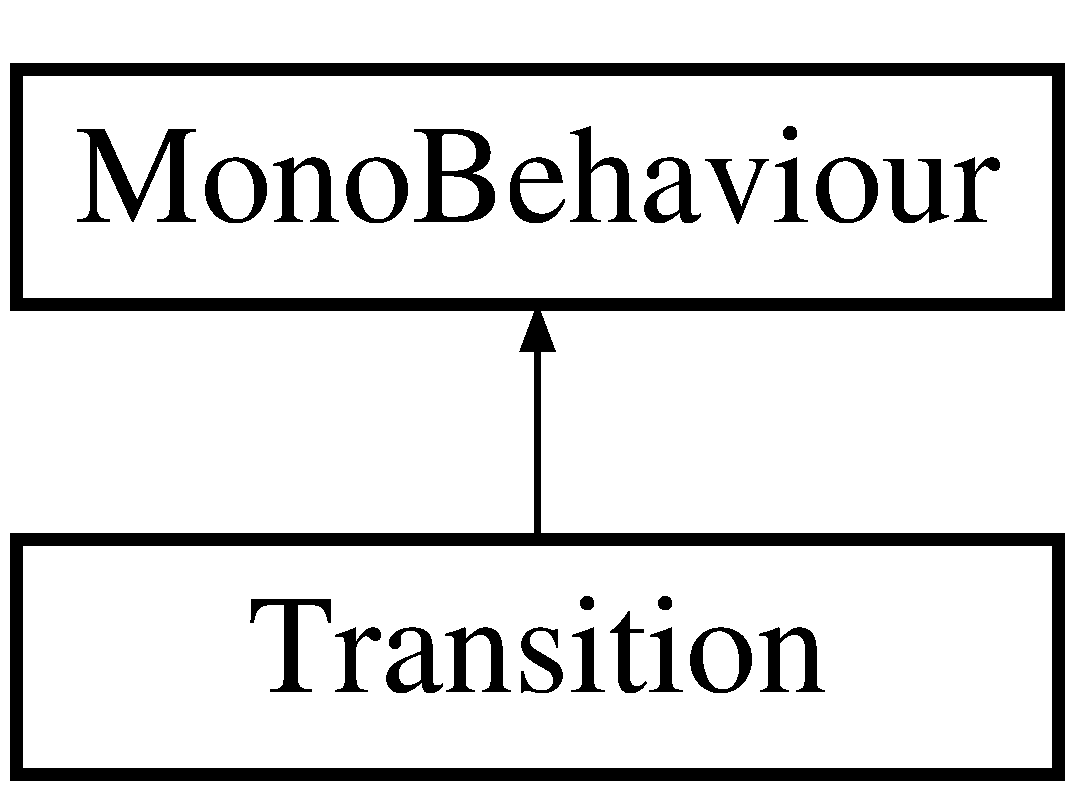
\includegraphics[height=2.000000cm]{class_transition}
\end{center}
\end{figure}
\subsection*{Public Member Functions}
\begin{DoxyCompactItemize}
\item 
void \hyperlink{class_transition_acab716cbd4bcbd3da46e1161cd2a43e2}{Exit\+Press} ()
\item 
void \hyperlink{class_transition_a10c8060f16a9b5d09ce4524b9f8efa0f}{No\+Press} ()
\item 
void \hyperlink{class_transition_a6d5791afbbe63424104a41705c2aadfc}{transition\+Scene} ()
\item 
void \hyperlink{class_transition_a77fc2840187cd5d6b28430e307ccbe1e}{transition\+Help} ()
\item 
void \hyperlink{class_transition_ad49e89dfdf52c7cda9d0cbbe4639d6e6}{quit\+Game} ()
\end{DoxyCompactItemize}
\subsection*{Public Attributes}
\begin{DoxyCompactItemize}
\item 
Canvas \hyperlink{class_transition_ab609cd1ff603a1b4f70d1c485f791ddc}{quit\+Menu}
\item 
Button \hyperlink{class_transition_a4a6526330da3604fee707638f5ca9926}{start\+Text}
\item 
Button \hyperlink{class_transition_adb5a3c819a57321e4e06e92cb17fdf02}{exit\+Text}
\end{DoxyCompactItemize}


\subsection{Detailed Description}


Definition at line 14 of file Transition.\+cs.



\subsection{Member Function Documentation}
\hypertarget{class_transition_acab716cbd4bcbd3da46e1161cd2a43e2}{}\label{class_transition_acab716cbd4bcbd3da46e1161cd2a43e2} 
\index{Transition@{Transition}!Exit\+Press@{Exit\+Press}}
\index{Exit\+Press@{Exit\+Press}!Transition@{Transition}}
\subsubsection{\texorpdfstring{Exit\+Press()}{ExitPress()}}
{\footnotesize\ttfamily void Transition.\+Exit\+Press (\begin{DoxyParamCaption}{ }\end{DoxyParamCaption})}

To enable quit menu if exit button is pressed from main menu. 

Definition at line 39 of file Transition.\+cs.

\hypertarget{class_transition_a10c8060f16a9b5d09ce4524b9f8efa0f}{}\label{class_transition_a10c8060f16a9b5d09ce4524b9f8efa0f} 
\index{Transition@{Transition}!No\+Press@{No\+Press}}
\index{No\+Press@{No\+Press}!Transition@{Transition}}
\subsubsection{\texorpdfstring{No\+Press()}{NoPress()}}
{\footnotesize\ttfamily void Transition.\+No\+Press (\begin{DoxyParamCaption}{ }\end{DoxyParamCaption})}

To disable quit menu if no button is pressed on said menu. 

Definition at line 49 of file Transition.\+cs.

\hypertarget{class_transition_ad49e89dfdf52c7cda9d0cbbe4639d6e6}{}\label{class_transition_ad49e89dfdf52c7cda9d0cbbe4639d6e6} 
\index{Transition@{Transition}!quit\+Game@{quit\+Game}}
\index{quit\+Game@{quit\+Game}!Transition@{Transition}}
\subsubsection{\texorpdfstring{quit\+Game()}{quitGame()}}
{\footnotesize\ttfamily void Transition.\+quit\+Game (\begin{DoxyParamCaption}{ }\end{DoxyParamCaption})}

End game function. 

Definition at line 75 of file Transition.\+cs.

\hypertarget{class_transition_a77fc2840187cd5d6b28430e307ccbe1e}{}\label{class_transition_a77fc2840187cd5d6b28430e307ccbe1e} 
\index{Transition@{Transition}!transition\+Help@{transition\+Help}}
\index{transition\+Help@{transition\+Help}!Transition@{Transition}}
\subsubsection{\texorpdfstring{transition\+Help()}{transitionHelp()}}
{\footnotesize\ttfamily void Transition.\+transition\+Help (\begin{DoxyParamCaption}{ }\end{DoxyParamCaption})}

\hyperlink{class_transition}{Transition} to help scene. 

Definition at line 67 of file Transition.\+cs.

\hypertarget{class_transition_a6d5791afbbe63424104a41705c2aadfc}{}\label{class_transition_a6d5791afbbe63424104a41705c2aadfc} 
\index{Transition@{Transition}!transition\+Scene@{transition\+Scene}}
\index{transition\+Scene@{transition\+Scene}!Transition@{Transition}}
\subsubsection{\texorpdfstring{transition\+Scene()}{transitionScene()}}
{\footnotesize\ttfamily void Transition.\+transition\+Scene (\begin{DoxyParamCaption}{ }\end{DoxyParamCaption})}

\hyperlink{class_transition}{Transition} to main scene. 

Definition at line 59 of file Transition.\+cs.



\subsection{Member Data Documentation}
\hypertarget{class_transition_adb5a3c819a57321e4e06e92cb17fdf02}{}\label{class_transition_adb5a3c819a57321e4e06e92cb17fdf02} 
\index{Transition@{Transition}!exit\+Text@{exit\+Text}}
\index{exit\+Text@{exit\+Text}!Transition@{Transition}}
\subsubsection{\texorpdfstring{exit\+Text}{exitText}}
{\footnotesize\ttfamily Button Transition.\+exit\+Text}



Definition at line 23 of file Transition.\+cs.

\hypertarget{class_transition_ab609cd1ff603a1b4f70d1c485f791ddc}{}\label{class_transition_ab609cd1ff603a1b4f70d1c485f791ddc} 
\index{Transition@{Transition}!quit\+Menu@{quit\+Menu}}
\index{quit\+Menu@{quit\+Menu}!Transition@{Transition}}
\subsubsection{\texorpdfstring{quit\+Menu}{quitMenu}}
{\footnotesize\ttfamily Canvas Transition.\+quit\+Menu}



Definition at line 17 of file Transition.\+cs.

\hypertarget{class_transition_a4a6526330da3604fee707638f5ca9926}{}\label{class_transition_a4a6526330da3604fee707638f5ca9926} 
\index{Transition@{Transition}!start\+Text@{start\+Text}}
\index{start\+Text@{start\+Text}!Transition@{Transition}}
\subsubsection{\texorpdfstring{start\+Text}{startText}}
{\footnotesize\ttfamily Button Transition.\+start\+Text}



Definition at line 20 of file Transition.\+cs.



The documentation for this class was generated from the following file\+:\begin{DoxyCompactItemize}
\item 
Virus\+Project/\+Assets/\+Scripts/\hyperlink{_transition_8cs}{Transition.\+cs}\end{DoxyCompactItemize}

\hypertarget{class_transition2}{}\section{Transition2 Class Reference}
\label{class_transition2}\index{Transition2@{Transition2}}
Inheritance diagram for Transition2\+:\begin{figure}[H]
\begin{center}
\leavevmode
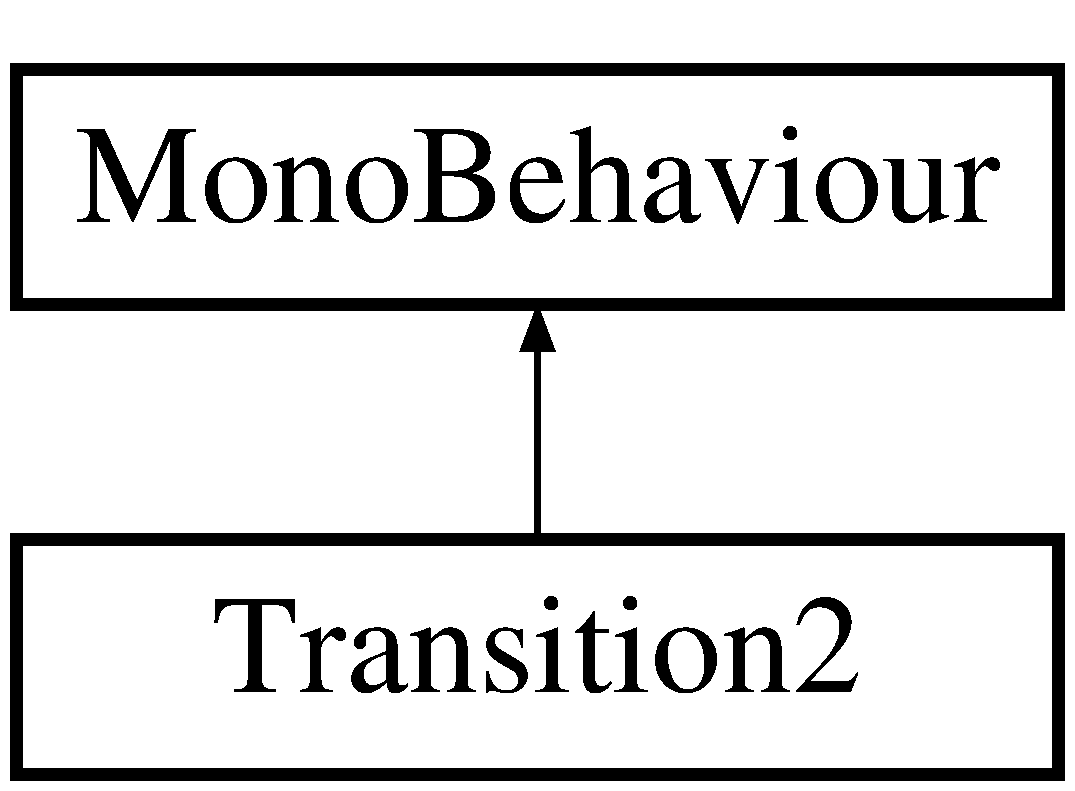
\includegraphics[height=2.000000cm]{class_transition2}
\end{center}
\end{figure}
\subsection*{Public Member Functions}
\begin{DoxyCompactItemize}
\item 
void \hyperlink{class_transition2_ac7ff3fc26ca27062e468add114ef890a}{Exit\+Press} ()
\item 
void \hyperlink{class_transition2_a3d85518cb434a02cf4635ff8fc1d4b65}{No\+Press} ()
\item 
void \hyperlink{class_transition2_a051383599c21c51604589cadec4bdcf1}{transition\+Scene} ()
\end{DoxyCompactItemize}
\subsection*{Public Attributes}
\begin{DoxyCompactItemize}
\item 
Canvas \hyperlink{class_transition2_a2f95f61b801d5c9995910a8c7b3ed48d}{quit\+Menu}
\end{DoxyCompactItemize}


\subsection{Detailed Description}


Definition at line 14 of file Transition2.\+cs.



\subsection{Member Function Documentation}
\hypertarget{class_transition2_ac7ff3fc26ca27062e468add114ef890a}{}\label{class_transition2_ac7ff3fc26ca27062e468add114ef890a} 
\index{Transition2@{Transition2}!Exit\+Press@{Exit\+Press}}
\index{Exit\+Press@{Exit\+Press}!Transition2@{Transition2}}
\subsubsection{\texorpdfstring{Exit\+Press()}{ExitPress()}}
{\footnotesize\ttfamily void Transition2.\+Exit\+Press (\begin{DoxyParamCaption}{ }\end{DoxyParamCaption})}

To enable quit menu if exit button is pressed from main menu. 

Definition at line 53 of file Transition2.\+cs.

\hypertarget{class_transition2_a3d85518cb434a02cf4635ff8fc1d4b65}{}\label{class_transition2_a3d85518cb434a02cf4635ff8fc1d4b65} 
\index{Transition2@{Transition2}!No\+Press@{No\+Press}}
\index{No\+Press@{No\+Press}!Transition2@{Transition2}}
\subsubsection{\texorpdfstring{No\+Press()}{NoPress()}}
{\footnotesize\ttfamily void Transition2.\+No\+Press (\begin{DoxyParamCaption}{ }\end{DoxyParamCaption})}

To disable quit menu if no button is pressed on said menu. 

Definition at line 61 of file Transition2.\+cs.

\hypertarget{class_transition2_a051383599c21c51604589cadec4bdcf1}{}\label{class_transition2_a051383599c21c51604589cadec4bdcf1} 
\index{Transition2@{Transition2}!transition\+Scene@{transition\+Scene}}
\index{transition\+Scene@{transition\+Scene}!Transition2@{Transition2}}
\subsubsection{\texorpdfstring{transition\+Scene()}{transitionScene()}}
{\footnotesize\ttfamily void Transition2.\+transition\+Scene (\begin{DoxyParamCaption}{ }\end{DoxyParamCaption})}

\hyperlink{class_transition}{Transition} to main menu scene. 

Definition at line 69 of file Transition2.\+cs.



\subsection{Member Data Documentation}
\hypertarget{class_transition2_a2f95f61b801d5c9995910a8c7b3ed48d}{}\label{class_transition2_a2f95f61b801d5c9995910a8c7b3ed48d} 
\index{Transition2@{Transition2}!quit\+Menu@{quit\+Menu}}
\index{quit\+Menu@{quit\+Menu}!Transition2@{Transition2}}
\subsubsection{\texorpdfstring{quit\+Menu}{quitMenu}}
{\footnotesize\ttfamily Canvas Transition2.\+quit\+Menu}



Definition at line 17 of file Transition2.\+cs.



The documentation for this class was generated from the following file\+:\begin{DoxyCompactItemize}
\item 
Virus\+Project/\+Assets/\+Scripts/\hyperlink{_transition2_8cs}{Transition2.\+cs}\end{DoxyCompactItemize}

\chapter{File Documentation}
\hypertarget{ai_anim_8cs}{}\section{Virus\+Project/\+Assets/\+Scripts/ai\+Anim.cs File Reference}
\label{ai_anim_8cs}\index{Virus\+Project/\+Assets/\+Scripts/ai\+Anim.\+cs@{Virus\+Project/\+Assets/\+Scripts/ai\+Anim.\+cs}}
\subsection*{Classes}
\begin{DoxyCompactItemize}
\item 
class \hyperlink{classai_anim}{ai\+Anim}
\end{DoxyCompactItemize}

\hypertarget{_camera_script_8cs}{}\section{Virus\+Project/\+Assets/\+Scripts/\+Camera\+Script.cs File Reference}
\label{_camera_script_8cs}\index{Virus\+Project/\+Assets/\+Scripts/\+Camera\+Script.\+cs@{Virus\+Project/\+Assets/\+Scripts/\+Camera\+Script.\+cs}}
\subsection*{Classes}
\begin{DoxyCompactItemize}
\item 
class \hyperlink{class_camera_script}{Camera\+Script}
\end{DoxyCompactItemize}

\hypertarget{destination_talk_8cs}{}\section{Virus\+Project/\+Assets/\+Scripts/destination\+Talk.cs File Reference}
\label{destination_talk_8cs}\index{Virus\+Project/\+Assets/\+Scripts/destination\+Talk.\+cs@{Virus\+Project/\+Assets/\+Scripts/destination\+Talk.\+cs}}
\subsection*{Classes}
\begin{DoxyCompactItemize}
\item 
class \hyperlink{classdestination_talk}{destination\+Talk}
\end{DoxyCompactItemize}

\hypertarget{_display_text_8cs}{}\section{Virus\+Project/\+Assets/\+Scripts/\+Display\+Text.cs File Reference}
\label{_display_text_8cs}\index{Virus\+Project/\+Assets/\+Scripts/\+Display\+Text.\+cs@{Virus\+Project/\+Assets/\+Scripts/\+Display\+Text.\+cs}}
\subsection*{Classes}
\begin{DoxyCompactItemize}
\item 
class \hyperlink{class_display_text}{Display\+Text}
\end{DoxyCompactItemize}

\hypertarget{face_mouse_8cs}{}\section{Virus\+Project/\+Assets/\+Scripts/face\+Mouse.cs File Reference}
\label{face_mouse_8cs}\index{Virus\+Project/\+Assets/\+Scripts/face\+Mouse.\+cs@{Virus\+Project/\+Assets/\+Scripts/face\+Mouse.\+cs}}
\subsection*{Classes}
\begin{DoxyCompactItemize}
\item 
class \hyperlink{classface_mouse}{face\+Mouse}
\end{DoxyCompactItemize}

\hypertarget{_game_manager_8cs}{}\section{Virus\+Project/\+Assets/\+Scripts/\+Game\+Manager.cs File Reference}
\label{_game_manager_8cs}\index{Virus\+Project/\+Assets/\+Scripts/\+Game\+Manager.\+cs@{Virus\+Project/\+Assets/\+Scripts/\+Game\+Manager.\+cs}}
\subsection*{Classes}
\begin{DoxyCompactItemize}
\item 
class \hyperlink{class_game_manager}{Game\+Manager}
\end{DoxyCompactItemize}

\hypertarget{_infection_8cs}{}\section{Virus\+Project/\+Assets/\+Scripts/\+Infection.cs File Reference}
\label{_infection_8cs}\index{Virus\+Project/\+Assets/\+Scripts/\+Infection.\+cs@{Virus\+Project/\+Assets/\+Scripts/\+Infection.\+cs}}
\subsection*{Classes}
\begin{DoxyCompactItemize}
\item 
class \hyperlink{class_infection}{Infection}
\end{DoxyCompactItemize}

\hypertarget{main_menu_8cs}{}\section{Virus\+Project/\+Assets/\+Scripts/main\+Menu.cs File Reference}
\label{main_menu_8cs}\index{Virus\+Project/\+Assets/\+Scripts/main\+Menu.\+cs@{Virus\+Project/\+Assets/\+Scripts/main\+Menu.\+cs}}
\subsection*{Classes}
\begin{DoxyCompactItemize}
\item 
class \hyperlink{classmain_menu}{main\+Menu}
\end{DoxyCompactItemize}

\hypertarget{_player_mobility_8cs}{}\section{Virus\+Project/\+Assets/\+Scripts/\+Player\+Mobility.cs File Reference}
\label{_player_mobility_8cs}\index{Virus\+Project/\+Assets/\+Scripts/\+Player\+Mobility.\+cs@{Virus\+Project/\+Assets/\+Scripts/\+Player\+Mobility.\+cs}}
\subsection*{Classes}
\begin{DoxyCompactItemize}
\item 
class \hyperlink{class_player_mobility}{Player\+Mobility}
\end{DoxyCompactItemize}

\hypertarget{sim_person_8cs}{}\section{Virus\+Project/\+Assets/\+Scripts/sim\+Person.cs File Reference}
\label{sim_person_8cs}\index{Virus\+Project/\+Assets/\+Scripts/sim\+Person.\+cs@{Virus\+Project/\+Assets/\+Scripts/sim\+Person.\+cs}}
\subsection*{Classes}
\begin{DoxyCompactItemize}
\item 
class \hyperlink{classsim_person}{sim\+Person}
\item 
class \hyperlink{classsim_person_1_1_dest_slot}{sim\+Person.\+Dest\+Slot}
\item 
class \hyperlink{classsim_person_1_1_my_state}{sim\+Person.\+My\+State}
\end{DoxyCompactItemize}

\hypertarget{_transition_8cs}{}\section{Virus\+Project/\+Assets/\+Scripts/\+Transition.cs File Reference}
\label{_transition_8cs}\index{Virus\+Project/\+Assets/\+Scripts/\+Transition.\+cs@{Virus\+Project/\+Assets/\+Scripts/\+Transition.\+cs}}
\subsection*{Classes}
\begin{DoxyCompactItemize}
\item 
class \hyperlink{class_transition}{Transition}
\end{DoxyCompactItemize}

\hypertarget{_transition2_8cs}{}\section{Virus\+Project/\+Assets/\+Scripts/\+Transition2.cs File Reference}
\label{_transition2_8cs}\index{Virus\+Project/\+Assets/\+Scripts/\+Transition2.\+cs@{Virus\+Project/\+Assets/\+Scripts/\+Transition2.\+cs}}
\subsection*{Classes}
\begin{DoxyCompactItemize}
\item 
class \hyperlink{class_transition2}{Transition2}
\end{DoxyCompactItemize}

%--- End generated contents ---

% Index
\backmatter
\newpage
\phantomsection
\clearemptydoublepage
\addcontentsline{toc}{chapter}{Index}
\printindex

\end{document}
